%%%%%%%%%%%%%%%%%%%%%%%%%%%%%%%%%%%%%%%%%%%%%%%%%%%%%%%%%%%%%%%%%%%%%%%%%%
% Modelo de Dissertacao de Mestrado PROCC/UFS
%%%%%%%%%%%%%%%%%%%%%%%%%%%%%%%%%%%%%%%%%%%%%%%%%%%%%%%%%%%%%%%%%%%%%%%%%%

\documentclass[english,
               brazilian,
               msc]
               {dcomp-abntex2}

%%%%%%%%%%%%%%%%%%%%%%%%%%%%%%%%%%%%%%%%%%%%%%%%%%%%%%%%%%%%%%%%%%%%%%%%%%
% Area para adicao de pacotes extras
% --- Pacotes mínimos necessários ---
\usepackage{float}
\usepackage{booktabs}
\usepackage{tabularx}
\usepackage{tikz}
\usetikzlibrary{arrows.meta,positioning,shapes.geometric,calc}
\usepackage{pgfplots}
\pgfplotsset{compat=1.18}
\usepackage{subcaption}
\usepackage{url}
\usepackage{footmisc}
\setlength{\footnotemargin}{1em}
\usepackage[table]{xcolor}

%\includegraphics.
%%%%%%%%%%%%%%%%%%%%%%%%%%%%%%%%%%%%%%%%%%%%%%%%%%%%%%%%%%%%%%%%%%%%%%%%%%
%%%%%%%%%%%%%%%%%%%%%%%%%%%%%%%%%%%%%%%%%%%%%%%%%%%%%%%%%%%%%%%%%%%%%%%%%%

% Utilize aqui seu pacote preferido para algoritmos.
\usepackage[linesnumbered]{algorithm2e}

%%%%%%%%%%%%%%%%%%%%%%%%%%%%%%%%%%%%%%%%%%%%%%%%%%%%%%%%%%%%%%%%%%%%%%%%%%

% Compila o indice.
\makeindex

\begin{document}

\hypersetup{hidelinks}
% Seleciona o idioma do documento (conforme pacotes do babel).
\selectlanguage{brazilian}

% Retira espaco extra obsoleto entre as frases.
\frenchspacing

%%%%%%%%%%%%%%%%%%%%%%%%%%%%%%%%%%%%%%%%%%%%%%%%%%%%%%%%%%%%%%%%%%%%%%%%%%
% ELEMENTOS PRE-TEXTUAIS
%%%%%%%%%%%%%%%%%%%%%%%%%%%%%%%%%%%%%%%%%%%%%%%%%%%%%%%%%%%%%%%%%%%%%%%%%%

\pretextual

\titulo{Tomada de Decisão Arquitetural em Sistemas Intensivos em Dados: uma abordagem baseada em evidências}
\autor{José Bruno Barros dos Santos}
\orientador{Fábio Gomes Rocha}
% \coorientador{Nome do Coorientador}
\curso{Ciência da Computação}

\inserirInformacoesPDF

\imprimircapa
\imprimirfolhaderosto*

%\include{Pre_Textual/Dedicatoria}
%\include{Pre_Textual/Agradecimentos}
\begin{epigrafe}
    \vspace*{\fill}
    \begin{flushright}
        \textit{We've always defined ourselves by the ability to overcome the impossible. And we count these moments. These moments when we dare to aim higher, to break barriers, to reach for the stars, to make the unknown known. We count these moments as our proudest achievements. But we lost all that. Or perhaps we've just forgotten that we are still pioneers. And we've barely begun. And that our greatest accomplishments cannot be behind us, because our destiny lies above us.
        (Interstellar)}
    \end{flushright}
\end{epigrafe}

% Resumo em portugues.
\setlength{\absparsep}{18pt}

\begin{resumo}
\textbf{Contexto:} Sistemas intensivos em dados são fundamentais para o processamento, armazenamento, movimentação e análise de grandes volumes de dados em infraestruturas modernas de software. Esses sistemas envolvem decisões arquiteturais relacionadas a paradigmas de processamento, ingestão de dados, escalabilidade, uso de recursos e tolerância a falhas, as quais impactam diretamente atributos como \textit{throughput}, latência, estabilidade e custo computacional. \textbf{Problema:} Apesar da existência de diferentes técnicas, \textit{frameworks} e estratégias de otimização para sistemas intensivos em dados, as evidências empíricas disponíveis na literatura permanecem fragmentadas, heterogêneas e, muitas vezes, difíceis de comparar. Essa limitação dificulta a tomada de decisão arquitetural baseada em evidências, especialmente em cenários que exigem a escolha entre processamento em lote, processamento em fluxo e diferentes configurações de execução. \textbf{Solução:} Esta pesquisa propõe investigar uma abordagem quantitativa de apoio à decisão arquitetural em sistemas intensivos em dados, integrando evidências da literatura, resultados experimentais e características observáveis dos dados, como volume, entropia, redundância, cardinalidade e variabilidade. \textbf{Método:} A pesquisa foi organizada em três etapas complementares: uma Revisão Sistemática da Literatura, uma campanha experimental controlada e a proposta de um modelo quantitativo de apoio à decisão arquitetural. A revisão sistemática identificou técnicas, métricas, lacunas e evidências relacionadas ao design de sistemas intensivos em dados. A campanha experimental comparou processamento \textit{batch} e \textit{streaming} em um ambiente baseado em Apache Spark, Spark Structured Streaming, Apache Kafka e Docker, utilizando o dataset NYC Taxi. Foram avaliados diferentes volumes de dados, taxas de eventos, números de \textit{workers} e intervalos de \textit{trigger}, considerando métricas como \textit{throughput}, latência, uso de CPU, consumo de memória, \textit{backpressure} e escalabilidade. \textbf{Sumarização dos resultados:} A revisão sistemática identificou 979 registros, dos quais dez estudos primários atenderam aos critérios de inclusão e qualidade. A síntese quantitativa exploratória indicou efeitos positivos de otimizações arquiteturais, com razão média de resposta de aproximadamente $2{,}7\times$ em relação às configurações de referência. Os resultados experimentais parciais indicaram que o processamento \textit{batch} apresentou maior \textit{throughput} nos cenários avaliados, enquanto o processamento \textit{streaming} mostrou maior sensibilidade à taxa de eventos, ao intervalo de \textit{trigger} e aos custos de coordenação dos micro-lotes. \textbf{Contribuição:} Espera-se que esta pesquisa contribua para a tomada de decisão arquitetural em sistemas intensivos em dados por meio de uma abordagem baseada em evidências empíricas, resultados experimentais e características informacionais dos dados, auxiliando arquitetos de software e engenheiros de dados na comparação preliminar entre alternativas arquiteturais antes da implementação completa de uma solução.

\textbf{Palavras-chave:} Sistemas Intensivos em Dados. Arquitetura de Software. Tomada de Decisão Arquitetural. Processamento em Fluxo. Teoria da Informação.


\end{resumo}

% Abstract in English.
\setlength{\absparsep}{18pt}
\begin{resumo}[Abstract]
\begin{otherlanguage*}{english}


\textbf{Context:} Data-intensive systems are fundamental for processing, storing, moving, and analyzing large volumes of data in modern software infrastructures. These systems involve architectural decisions related to processing paradigms, data ingestion, scalability, resource usage, and fault tolerance, which directly impact attributes such as \textit{throughput}, latency, stability, and computational cost. \textbf{Problem:} Despite the existence of different techniques, \textit{frameworks}, and optimization strategies for data-intensive systems, the empirical evidence available in the literature remains fragmented, heterogeneous, and often difficult to compare. This limitation makes evidence-based architectural decision-making difficult, especially in scenarios that require choosing between batch processing, stream processing, and different execution configurations. \textbf{Solution:} This research proposes to investigate a quantitative approach to support architectural decision-making in data-intensive systems by integrating evidence from the literature, experimental results, and observable data characteristics, such as volume, entropy, redundancy, cardinality, and variability. \textbf{Method:} The research was organized into three complementary stages: a Systematic Literature Review, a controlled experimental campaign, and the proposal of a quantitative model to support architectural decision-making. The systematic review identified techniques, metrics, gaps, and evidence related to the design of data-intensive systems. The experimental campaign compared \textit{batch} and \textit{streaming} processing in an environment based on Apache Spark, Spark Structured Streaming, Apache Kafka, and Docker, using the NYC Taxi dataset. Different data volumes, event rates, numbers of \textit{workers}, and \textit{trigger} intervals were evaluated, considering metrics such as \textit{throughput}, latency, CPU usage, memory consumption, \textit{backpressure}, and scalability. \textbf{Summary of results:} The systematic review identified 979 records, of which ten primary studies met the inclusion and quality criteria. The exploratory quantitative synthesis indicated positive effects of architectural optimizations, with an average response ratio of approximately $2.7\times$ compared to baseline configurations. The preliminary experimental results indicated that \textit{batch} processing achieved higher \textit{throughput} in the evaluated scenarios, while \textit{streaming} processing showed greater sensitivity to event rate, \textit{trigger} interval, and micro-batch coordination costs. \textbf{Contribution:} This research is expected to contribute to architectural decision-making in data-intensive systems through an approach based on empirical evidence, experimental results, and informational characteristics of data, supporting software architects and data engineers in the preliminary comparison of architectural alternatives before the complete implementation of a solution.

\textbf{Keywords:} Data-Intensive Systems. Software Architecture. Architectural Decision-Making. Stream Processing. Information Theory.



\end{otherlanguage*}
\end{resumo}


\mostrarlistadeILUSTRACOES
%\mostrarlistadeQUADROS
\mostrarlistadeTABELAS
%\mostrarlistadeCODIGOS
%\mostrarlistadeALGORITMOS

\begin{siglas}
\item[ABNT]{Associação Brasileira de Normas Técnicas}
\item[ACM]{Association for Computing Machinery}
\item[API]{Application Programming Interface}
\item[CPU]{Central Processing Unit}
\item[CSV]{Comma-Separated Values}
\item[GB]{Gigabyte}
\item[HPC]{High Performance Computing}
\item[IEEE]{Institute of Electrical and Electronics Engineers}
\item[IoT]{Internet of Things}
\item[LRR]{Log Response Ratio}
\item[MB]{Megabyte}
\item[NDP]{Near-Data Processing}
\item[NVM]{Non-Volatile Memory}
\item[NYC]{New York City}
\item[PRISMA]{Preferred Reporting Items for Systematic Reviews and Meta-Analyses}
\item[PROCC]{Programa de Pós-Graduação em Ciência da Computação}
\item[QA]{Quality Assessment}
\item[RSL]{Revisão Sistemática da Literatura}
\item[SGBD]{Sistema de Gerenciamento de Banco de Dados}
\item[SQL]{Structured Query Language}
\item[UFS]{Universidade Federal de Sergipe}
\item[WEBIST]{International Conference on Web Information Systems and Technologies}
\item[YARN]{Yet Another Resource Negotiator}
\end{siglas}

\begin{simbolos}
   
\item[$X$] Variável aleatória discreta associada a um atributo, evento ou conjunto de valores analisado.

\item[$x_i$] Valor possível assumido pela variável aleatória $X$.

\item[$p(x_i)$] Probabilidade de ocorrência do valor $x_i$.

\item[$H(X)$] Entropia da variável aleatória $X$.

\item[$H_{max}(X)$] Entropia máxima possível da variável aleatória $X$.

\item[$R(X)$] Redundância associada à variável aleatória $X$.

\item[$C_D$] Vetor de características de um cenário de dados ou fluxo de eventos.

\item[$V$] Volume de dados considerado em um cenário experimental.

\item[$\lambda$] Taxa de chegada de eventos em um fluxo de dados.

\item[$K$] Cardinalidade de um atributo ou conjunto de dados.

\item[$\sigma$] Variabilidade temporal dos dados ou eventos.

\item[$L_{req}$] Restrição de latência requerida para um cenário.

\item[$A$] Conjunto de alternativas arquiteturais disponíveis.

\item[$a$] Alternativa arquitetural pertencente ao conjunto $A$.

\item[$P_a$] Vetor de desempenho associado à alternativa arquitetural $a$.

\item[$T_a$] \textit{Throughput} observado ou estimado para a alternativa $a$.

\item[$L_a$] Latência observada ou estimada para a alternativa $a$.

\item[$U_{cpu,a}$] Uso de CPU associado à alternativa arquitetural $a$.

\item[$U_{mem,a}$] Consumo de memória associado à alternativa arquitetural $a$.

\item[$B_a$] Nível de \textit{backpressure} associado à alternativa arquitetural $a$.

\item[$E_a$] Indicador de eficiência ou estabilidade associado à alternativa arquitetural $a$.

\item[$S(a)$] Escore de adequação atribuído à alternativa arquitetural $a$.

\item[$w_i$] Peso atribuído ao critério $i$ em uma função de decisão.

\item[$RR_i$] Razão de resposta do estudo ou cenário $i$.

\item[$LRR_i$] Razão de resposta logarítmica do estudo ou cenário $i$.

\item[$\overline{LRR}$] Média dos valores de Razão de Resposta Logarítmica.

\item[$k$] Número de estudos incluídos na síntese quantitativa.

\item[$M_{tratamento}$] Valor da métrica observado na configuração otimizada ou experimental.

\item[$M_{baseline}$] Valor da métrica observado na configuração de referência.

\item[$N_{registros}$] Número de registros processados em uma execução experimental.

\item[$T_{processamento}$] Tempo total de processamento de uma execução experimental.

\item[$\delta$] Tamanho de efeito de Cliff's Delta.


\end{simbolos}


\mostrarSUMARIO

%%%%%%%%%%%%%%%%%%%%%%%%%%%%%%%%%%%%%%%%%%%%%%%%%%%%%%%%%%%%%%%%%%%%%%%%%%
% ELEMENTOS TEXTUAIS
%%%%%%%%%%%%%%%%%%%%%%%%%%%%%%%%%%%%%%%%%%%%%%%%%%%%%%%%%%%%%%%%%%%%%%%%%%

\textual
\chapter{Introdução}
\label{cap:introducao}

A crescente digitalização de processos sociais, científicos, industriais e organizacionais tem provocado um aumento contínuo na produção, armazenamento, transmissão e processamento de dados. Esse cenário intensifica a relevância dos sistemas intensivos em dados, isto é, sistemas projetados para lidar com grandes volumes de dados, múltiplas fontes de informação, diferentes formatos e requisitos rigorosos de desempenho, escalabilidade, disponibilidade e confiabilidade. Em ambientes de Big Data, esses desafios são frequentemente associados às características de volume, velocidade, variedade e veracidade dos dados, as quais influenciam diretamente o modo como as arquiteturas de software são concebidas e avaliadas \cite{dai2019big,hilbert2016big}.

Diferentemente de sistemas tradicionais, aplicações intensivas em dados dependem da integração entre componentes distribuídos, mecanismos de armazenamento, plataformas de processamento paralelo, sistemas de mensageria, estratégias de movimentação de dados e técnicas de gerenciamento de recursos. Nesse contexto, decisões arquiteturais deixam de ser apenas escolhas estruturais de alto nível e passam a exercer impacto direto sobre atributos de qualidade, como latência, \textit{throughput}, escalabilidade, tolerância a falhas e eficiência no uso de recursos computacionais \cite{mattmann2004software,ji2020quality,kleppmann2017designing}.

Entre as decisões arquiteturais mais relevantes nesse domínio, destacam-se aquelas relacionadas à forma como os dados são ingeridos, movimentados, armazenados e processados ao longo de um \textit{pipeline}. A escolha entre processamento em lote (\textit{batch processing}) e processamento em fluxo (\textit{stream processing}), por exemplo, pode alterar substancialmente o comportamento do sistema em termos de vazão, tempo de resposta, estabilidade temporal e consumo de recursos. Do mesmo modo, decisões sobre particionamento, escalonamento, localização do processamento, uso de memória, transferência entre sistemas e configuração de mecanismos de tolerância a falhas podem produzir impactos distintos conforme o volume dos dados, a taxa de chegada dos eventos e o ambiente de execução \cite{haynes2016pipegen,wang2018hard,aung2019coordinate,lyu2022fine}.

Apesar da existência de diversas técnicas, \textit{frameworks} e estratégias voltadas à otimização de sistemas intensivos em dados, a literatura ainda apresenta evidências empíricas fragmentadas. Muitos estudos avaliam soluções específicas em contextos particulares, utilizando métricas, \textit{workloads} e ambientes experimentais heterogêneos. Essa fragmentação dificulta a comparação entre abordagens, reduz a capacidade de generalização dos resultados e limita o apoio sistemático à tomada de decisão arquitetural. Como consequência, arquitetos de software frequentemente precisam decidir entre alternativas tecnológicas e arquiteturais com base em experiências prévias, recomendações práticas ou experimentos isolados, sem dispor de mecanismos quantitativos capazes de orientar essas escolhas de forma mais objetiva.

Diante desse contexto, esta pesquisa parte do seguinte problema: como apoiar, de forma sistemática e baseada em evidências, a tomada de decisão arquitetural em sistemas intensivos em dados, considerando características dos dados, estratégias de processamento e métricas observáveis de desempenho?

Para enfrentar essa lacuna, a pesquisa foi organizada em três movimentos complementares. O primeiro consistiu na realização de uma Revisão Sistemática da Literatura sobre o \textit{design} de sistemas intensivos em dados, acompanhada de uma síntese quantitativa exploratória. Essa etapa permitiu identificar técnicas arquiteturais recorrentes, métricas utilizadas na avaliação de desempenho, padrões de otimização e lacunas metodológicas relacionadas ao relato experimental.

O segundo movimento consistiu na condução de uma campanha experimental voltada à produção de evidência empírica controlada sobre decisões arquiteturais em sistemas intensivos em dados. O experimento comparou os paradigmas de processamento \textit{batch} e \textit{streaming} utilizando tecnologias amplamente adotadas, como Apache Spark, Spark Structured Streaming e Apache Kafka. Foram avaliados diferentes volumes de dados, taxas de eventos, números de \textit{workers} e configurações de \textit{trigger}, considerando métricas como \textit{throughput}, latência, uso de CPU, consumo de memória, \textit{backpressure} e taxa de processamento \cite{zaharia2016apache,armbrust2018structured,kreps2011kafka,matteussi2022performance}.

Os resultados experimentais obtidos reforçam a importância de compreender os \textit{trade-offs} envolvidos nas decisões arquiteturais. O processamento \textit{batch} tende a favorecer maiores taxas de \textit{throughput} em determinados cenários, enquanto o processamento em fluxo introduz custos associados à ingestão contínua, à coordenação dos micro-lotes e ao controle de estabilidade temporal. Além disso, fatores como volume de dados, paralelismo horizontal e intervalo de \textit{trigger} podem alterar significativamente o comportamento do sistema, indicando que decisões arquiteturais devem ser analisadas de forma contextualizada e baseada em evidências.

O terceiro movimento da pesquisa consiste na proposta de uma abordagem quantitativa de apoio à decisão arquitetural, considerando evidências empíricas e características informacionais dos dados. A intenção é investigar se propriedades como volume, taxa de eventos, entropia, redundância e variabilidade podem ser combinadas com métricas de desempenho para apoiar a comparação entre alternativas arquiteturais.


A Figura~\ref{fig:fluxo-pesquisa} apresenta o encadeamento geral da pesquisa.

\begin{figure}[htbp]
\centering
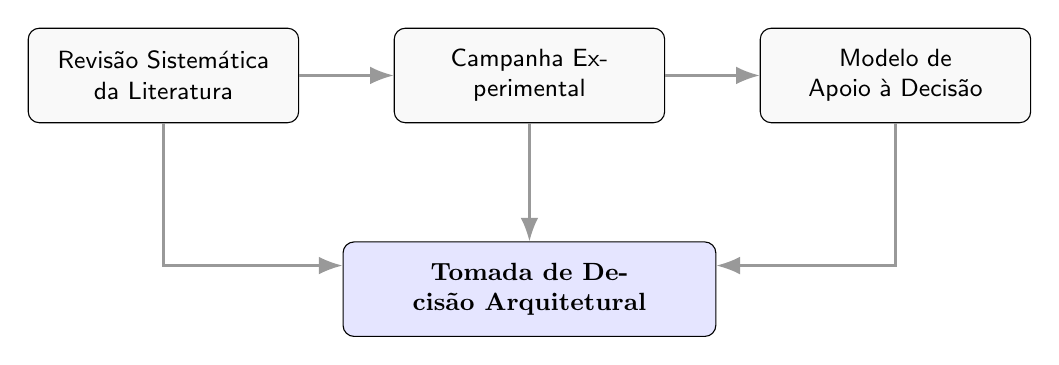
\begin{tikzpicture}[
    node distance=1.2cm and 1.2cm,
    etapa/.style={
        rectangle, rounded corners, draw, align=center,
        text width=3.2cm, minimum height=1.2cm,
        font=\small\sffamily, fill=gray!5
    },
    destaque/.style={
        etapa, font=\small\bfseries, fill=blue!10, text width=4.5cm
    },
    seta/.style={-{Latex[length=3mm]}, thick, draw=gray!80}
]

% Nós
\node[etapa] (rsl) {Revisão Sistemática da Literatura};
\node[etapa, right=of rsl] (exp) {Campanha Experimental};
\node[etapa, right=of exp] (modelo) {Modelo de Apoio à Decisão};
\node[destaque, below=1.5cm of exp] (decisao) {Tomada de Decisão Arquitetural};

% Conexões
\draw[seta] (rsl) -- (exp);
\draw[seta] (exp) -- (modelo);
\draw[seta] (rsl.south) |- ([yshift=0.3cm]decisao.west);
\draw[seta] (exp.south) -- (decisao.north);
\draw[seta] (modelo.south) |- ([yshift=0.3cm]decisao.east);

\end{tikzpicture}
\caption{Encadeamento conceitual da pesquisa.}
\label{fig:fluxo-pesquisa}
\end{figure}

\section{Objetivos}
\label{sec:intro-objetivos}

O objetivo geral desta pesquisa é investigar como evidências provenientes da literatura científica, resultados experimentais e características observáveis dos dados podem ser integrados para apoiar a tomada de decisão arquitetural em sistemas intensivos em dados.

Para alcançar esse objetivo geral, foram definidos os seguintes objetivos específicos:

\begin{enumerate}
\item caracterizar, por meio de uma Revisão Sistemática da Literatura, as principais técnicas, abordagens, métricas e lacunas relacionadas ao design de sistemas intensivos em dados;


\item sintetizar evidências quantitativas sobre o impacto de otimizações arquiteturais e sistêmicas no desempenho de sistemas intensivos em dados;

\item projetar e executar uma campanha experimental para comparar estratégias de processamento \textit{batch} e \textit{streaming} sob diferentes condições operacionais;

\item analisar estatisticamente os resultados experimentais, considerando métricas como \textit{throughput}, latência, escalabilidade, uso de recursos e estabilidade do processamento;

\item propor uma abordagem quantitativa de apoio à decisão arquitetural que relacione características dos dados e do processamento ao comportamento esperado do sistema.


\end{enumerate}

A justificativa desta pesquisa reside na necessidade de reduzir a dependência exclusiva de avaliações empíricas isoladas no processo de decisão arquitetural. Em sistemas intensivos em dados, a realização de experimentos completos para cada alternativa arquitetural pode demandar tempo, infraestrutura computacional e esforço de implementação significativos. Dessa forma, uma abordagem baseada em evidências pode auxiliar arquitetos de software na análise preliminar de alternativas, contribuindo para decisões mais fundamentadas, rastreáveis e alinhadas aos requisitos de desempenho e escalabilidade do sistema.

Além disso, esta pesquisa contribui para a área de Engenharia de Software ao aproximar três dimensões complementares: a consolidação de evidências científicas por meio de revisão sistemática, a produção de evidências empíricas por meio de experimentação controlada e a construção de mecanismos quantitativos para apoiar decisões arquiteturais. Essa integração busca avançar o conhecimento sobre o design de sistemas intensivos em dados e fornecer subsídios para pesquisas futuras relacionadas à avaliação, predição e recomendação de arquiteturas orientadas ao processamento intensivo de dados.


Esta proposta está organizada em oito capítulos. O Capítulo~\ref{cap:fundamentacao} apresenta a fundamentação teórica relacionada a sistemas intensivos em dados, decisões arquiteturais, processamento \textit{batch} e \textit{streaming}, Apache Spark, Apache Kafka e Teoria da Informação. O Capítulo~\ref{cap:metodologia} descreve a metodologia da pesquisa. O Capítulo~\ref{cap:rsl} apresenta a Revisão Sistemática da Literatura conduzida nesta pesquisa. O Capítulo~\ref{cap:campanha-experimental} descreve a campanha experimental realizada. O Capítulo~\ref{cap:resultados} apresenta os resultados parciais. O Capítulo~\ref{cap:cronograma} apresenta o cronograma da pesquisa. Por fim, o Capítulo~\ref{cap:proximos-passos} descreve os próximos passos e as atividades previstas para continuidade da dissertação.

\chapter{Fundamentação Teórica}
\label{cap:fundamentacao}

Os fundamentos conceituais que sustentam a pesquisa envolvem sistemas intensivos em dados, decisões arquiteturais e estratégias de processamento em larga escala. Inicialmente, discutem-se os sistemas intensivos em dados e sua relação com decisões arquiteturais. Em seguida, examinam-se os paradigmas de processamento em lote e processamento em fluxo, com ênfase em seus principais \textit{trade-offs}. Também são abordadas as tecnologias utilizadas na campanha experimental, especialmente Apache Spark, Spark Structured Streaming e Apache Kafka. Por fim, discutem-se as métricas de desempenho consideradas na avaliação experimental e os conceitos da Teoria da Informação que fundamentam a proposta de apoio à decisão arquitetural.

\section{Sistemas Intensivos em Dados e Decisões Arquiteturais}
\label{sec:sistemas-decisoes}

Sistemas intensivos em dados são sistemas de software cujo funcionamento depende fortemente da coleta, armazenamento, processamento, movimentação e análise de grandes volumes de dados. Esses sistemas são caracterizados não apenas pela quantidade de dados manipulada, mas também pela diversidade de formatos, pela velocidade com que os dados são produzidos e pela necessidade de manter níveis aceitáveis de desempenho, escalabilidade, confiabilidade e disponibilidade.

O crescimento de aplicações em domínios como computação em nuvem, Internet das Coisas (IoT), ciência de dados, sistemas de recomendação, monitoramento em tempo real e análise de grandes volumes de registros operacionais ampliou a importância desse tipo de sistema. Em tais contextos, os dados passam a ocupar papel central na arquitetura, influenciando decisões sobre armazenamento, particionamento, replicação, processamento, integração entre componentes e comunicação entre serviços \cite{dai2019big,hilbert2016big,kleppmann2017designing}.

Diferentemente de sistemas transacionais tradicionais, nos quais a lógica de negócio pode ocupar papel predominante na estrutura arquitetural, sistemas intensivos em dados exigem atenção especial ao fluxo dos dados ao longo da arquitetura. A forma como os dados são ingeridos, transformados, transportados e persistidos pode afetar diretamente atributos de qualidade. Por esse motivo, decisões arquiteturais nesse tipo de sistema devem considerar tanto os requisitos funcionais quanto os requisitos de qualidade associados ao comportamento operacional da aplicação \cite{mattmann2004software,ji2020quality}.

Decisões arquiteturais correspondem a escolhas de projeto que afetam a estrutura, o comportamento e os atributos de qualidade de um sistema de software. Em sistemas intensivos em dados, essas decisões envolvem, entre outros aspectos, a escolha de estratégias de processamento, mecanismos de armazenamento, formas de particionamento, políticas de replicação, tecnologias de mensageria, modelos de consistência, escalonamento de tarefas e alocação de recursos computacionais.

Essas decisões são críticas porque impactam diretamente características como latência, \textit{throughput}, escalabilidade, custo computacional, tolerância a falhas e eficiência no uso de CPU, memória, disco e rede. Por exemplo, uma arquitetura pode priorizar maior vazão em processamento em lote, enquanto outra pode priorizar menor latência e maior responsividade em processamento contínuo. Da mesma forma, uma estratégia de movimentação de dados pode reduzir o tempo de transferência entre sistemas, enquanto uma estratégia de processamento próximo aos dados pode reduzir custos de I/O e melhorar a escalabilidade \cite{haynes2016pipegen,vincon2020nkv}.

A literatura apresenta diferentes propostas voltadas à otimização de aspectos específicos dessas arquiteturas. Há estudos relacionados à otimização de escalonamento em ambientes Spark sobre YARN \cite{wang2018hard}, à compilação dinâmica de consultas SQL em Apache Spark \cite{schiavio2020dynamic}, ao gerenciamento fino de recursos em ambientes de Big Data \cite{lyu2022fine}, ao uso de armazenamento sensível a NVM para cargas analíticas \cite{gotze2018nvm-aware} e à ingestão transacional escalável de dados \cite{li2022karst}. Embora esses estudos apresentem contribuições relevantes, muitos deles avaliam soluções em contextos específicos, com métricas e configurações experimentais distintas.

Essa heterogeneidade torna a tomada de decisão arquitetural uma tarefa complexa. Arquitetos de software precisam escolher entre alternativas que podem apresentar vantagens em determinados cenários e limitações em outros. Assim, uma decisão adequada depende não apenas do conhecimento sobre tecnologias disponíveis, mas também da compreensão dos dados, da carga de trabalho, dos requisitos de desempenho e das restrições operacionais do ambiente.

\section{Processamento em Lote e Processamento em Fluxo}
\label{sec:batch-streaming}

Entre as decisões arquiteturais mais relevantes em sistemas intensivos em dados está a escolha entre processamento em lote e processamento em fluxo. O processamento em lote, ou \textit{batch processing}, consiste na execução de tarefas sobre conjuntos de dados previamente armazenados. Esse paradigma é amplamente utilizado em análises periódicas, geração de relatórios, processamento histórico e execução de cargas analíticas sobre grandes volumes de dados.

O processamento em fluxo, ou \textit{stream processing}, por sua vez, é orientado ao processamento contínuo de eventos à medida que eles são produzidos. Esse paradigma é especialmente relevante em cenários que exigem respostas próximas ao tempo real, como monitoramento de sensores, análise de \textit{logs}, detecção de anomalias, rastreamento de atividades e integração contínua de eventos em \textit{pipelines} de dados \cite{nasiri2019evaluation,armbrust2018structured}.

A escolha entre esses paradigmas envolve \textit{trade-offs}. O processamento em lote pode se beneficiar da disponibilidade de todo o conjunto de dados antes da execução, permitindo otimizações globais, melhor amortização de custos fixos e maior aproveitamento de recursos em determinados cenários. Por outro lado, esse paradigma pode não ser adequado para aplicações que exigem baixa latência ou resposta contínua a eventos.

O processamento em fluxo reduz o intervalo entre a chegada dos dados e sua análise, mas introduz desafios adicionais. Entre eles estão a necessidade de lidar com ingestão contínua, controle de atrasos, variação na taxa de eventos, tolerância a falhas, gerenciamento de estado, pressão de retorno (\textit{backpressure}) e estabilidade temporal do \textit{pipeline}. Em \textit{frameworks} baseados em micro-lotes, como o Spark Structured Streaming, o intervalo de \textit{trigger} também influencia o comportamento do sistema, afetando latência, \textit{throughput} e variabilidade do processamento \cite{armbrust2018structured,ivanov2018exploratory,matteussi2022performance}.

A literatura sobre processamento de fluxos mostra que sistemas baseados em micro-lotes e sistemas de processamento contínuo apresentam compromissos distintos. Sistemas de micro-lotes tendem a simplificar mecanismos de tolerância a falhas e integração com processamento em lote, mas podem introduzir maior latência em função do agrupamento dos dados em intervalos discretos. Sistemas contínuos podem alcançar menor latência, porém geralmente envolvem maior complexidade no controle de estado, recuperação e adaptação a falhas \cite{venkataraman2017drizzle}.


\section{Apache Spark, Spark Structured Streaming e Apache Kafka}
\label{sec:tecnologias}

A campanha experimental desta pesquisa utiliza tecnologias amplamente empregadas em arquiteturas de processamento distribuído e ingestão de dados. Entre elas, destacam-se o Apache Spark, o Spark Structured Streaming e o Apache Kafka.

O Apache Spark é um \textit{framework} de processamento distribuído projetado para executar aplicações de dados em larga escala sobre \textit{clusters} computacionais. Sua arquitetura oferece suporte a diferentes tipos de carga, incluindo processamento em lote, consultas SQL, aprendizado de máquina, processamento de grafos e processamento de fluxos de dados. O Spark tornou-se uma das plataformas mais utilizadas para processamento distribuído devido à sua flexibilidade, ao uso de abstrações de alto nível e à integração com diferentes formatos e fontes de dados \cite{zaharia2016apache,shanahan2015large}.

No contexto do processamento em lote, o Spark permite executar operações distribuídas sobre grandes conjuntos de dados, explorando paralelismo e distribuição de tarefas entre múltiplos nós do \textit{cluster}. Estudos mostram que o volume de dados, o número de recursos disponíveis e a configuração do ambiente podem afetar significativamente o desempenho de aplicações baseadas em Spark \cite{awan2015data,ahmed2020comprehensive}.

Além do volume de dados, a alocação de recursos computacionais é um fator relevante para o desempenho de aplicações Spark. A quantidade de memória atribuída aos executores, o número de núcleos, o número de nós, o paralelismo e a configuração do ambiente podem influenciar o tempo de execução, utilização média dos nós, gargalos de memória, operações de I/O e coleta de lixo (\textit{garbage collection}). Estudos experimentais indicam que diferentes combinações de tamanho dos dados, número de nós e recursos dos executores podem exigir configurações distintas para alcançar melhores resultados \cite{alcantara2019performance,shyamasundar2019fine}.

O Spark Structured Streaming estende o modelo do Spark para aplicações de processamento contínuo. Sua principal característica é oferecer uma API declarativa para fluxos de dados, permitindo que consultas sobre dados em tempo real sejam expressas de maneira semelhante a consultas sobre dados estáticos. Internamente, o Structured Streaming utiliza um modelo baseado em micro-lotes, no qual os dados recebidos são agrupados em pequenos intervalos de tempo e processados de forma incremental \cite{armbrust2018structured}.

Esse modelo simplifica o desenvolvimento de aplicações de \textit{streaming}, mas também introduz custos associados à coordenação dos micro-lotes, ao gerenciamento de estado, ao controle do intervalo de \textit{trigger} e à sincronização entre componentes. Por isso, a configuração adequada do ambiente e dos parâmetros de execução é essencial para alcançar o equilíbrio entre \textit{throughput}, latência e estabilidade do processamento. Estudos exploratórios sobre Spark Structured Streaming mostram que fatores como variação de volume, velocidade dos dados, número de consultas paralelas e intervalo de processamento podem alterar o comportamento do sistema \cite{ivanov2018exploratory}.

O Apache Kafka, por sua vez, é um sistema distribuído de mensageria baseado em \textit{log}, projetado para ingestão, armazenamento temporário e distribuição de fluxos de eventos em larga escala. O Kafka organiza mensagens em tópicos particionados, permitindo que produtores publiquem eventos e consumidores os leiam de forma escalável e desacoplada. Essa arquitetura favorece a construção de \textit{pipelines} de dados distribuídos, nos quais diferentes componentes podem produzir e consumir eventos de maneira independente \cite{kreps2011kafka}.

Em sistemas intensivos em dados, o Kafka é frequentemente utilizado como camada de ingestão e transporte de eventos. Sua capacidade de lidar com altas taxas de mensagens, particionamento e replicação o torna adequado para arquiteturas orientadas a eventos e \textit{pipelines} de processamento em fluxo. No entanto, seu uso também envolve decisões relacionadas ao número de partições, replicação, taxa de produção, consumo, persistência, tolerância a falhas e integração com \textit{frameworks} de processamento.

A confiabilidade em \textit{pipelines} baseados em Kafka pode ser influenciada por mecanismos de \textit{checkpoint}, replicação e recuperação após falhas. Estudos sobre arquiteturas de \textit{pipelines} Kafka indicam que mecanismos de \textit{checkpoint} podem reduzir o tempo de recuperação e perdas de mensagens em cenários de falha, reforçando a importância de decisões arquiteturais relacionadas à tolerância a falhas em sistemas de processamento contínuo \cite{aung2019coordinate}.

\section{Métricas de Desempenho}
\label{sec:metricas-desempenho}

A avaliação de sistemas intensivos em dados depende da definição de métricas capazes de representar o comportamento do sistema sob diferentes condições operacionais. Entre as métricas mais utilizadas estão \textit{throughput}, latência, tempo total de execução, uso de CPU, consumo de memória, utilização de disco, tráfego de rede, taxa de processamento e indicadores de estabilidade.

O \textit{throughput} representa a quantidade de dados processada por unidade de tempo. Em experimentos com processamento de dados, essa métrica pode ser expressa, por exemplo, em linhas por segundo, eventos por segundo ou \textit{bytes} por segundo. A latência, por sua vez, representa o tempo necessário para que um dado evento seja processado ou para que uma operação produza resultado. Em sistemas de \textit{streaming}, a latência pode ser analisada considerando o tempo entre a chegada do evento e seu processamento efetivo.

O uso de CPU e memória permite avaliar a eficiência do sistema em relação aos recursos computacionais disponíveis. Em ambientes distribuídos, tais métricas são importantes para compreender se o aumento do paralelismo resulta em ganhos efetivos ou se introduz \textit{overhead} de coordenação. Além disso, em \textit{pipelines} de \textit{streaming}, o \textit{backpressure} representa um indicador relevante de sobrecarga, pois indica a incapacidade temporária do sistema de acompanhar a taxa de chegada dos dados.

A literatura mostra que a avaliação de \textit{frameworks} distribuídos frequentemente considera métricas como tempo de execução, utilização de recursos, escalabilidade horizontal, escalabilidade vertical e custo. Em ambientes de nuvem e processamento distribuído, essas métricas ajudam a compreender não apenas o desempenho bruto do sistema, mas também sua eficiência operacional diante de diferentes configurações de infraestrutura \cite{ullah2022evaluation}.

No contexto específico de Spark e Spark Streaming, métricas como tempo de execução, \textit{throughput}, \textit{speedup}, uso de memória, utilização de CPU, latência e \textit{backpressure} são recorrentes em estudos experimentais. Pesquisas sobre desempenho em Spark indicam que o aumento do volume de dados pode intensificar custos de I/O, uso de memória e \textit{garbage collection}, enquanto estudos sobre \textit{streaming} mostram que variações na taxa de chegada dos eventos e na capacidade de processamento podem afetar diretamente a estabilidade do \textit{pipeline} \cite{awan2015data,ahmed2020comprehensive,matteussi2022performance}.

A Tabela~\ref{tab:metricas-desempenho} apresenta uma síntese das principais métricas consideradas nesta pesquisa.


\begin{table}[htbp]
\centering
\caption{Principais métricas de desempenho consideradas na pesquisa}
\label{tab:metricas-desempenho}
\renewcommand{\arraystretch}{1.2} 
\begin{tabularx}{\textwidth}{l l X}
\toprule
\textbf{Categoria} & \textbf{Métrica} & \textbf{Foco da Avaliação} \\ 
\midrule
Desempenho & \textit{Throughput} & Taxa de processamento por unidade de tempo (ex: eventos/s). \\ 
           & Latência & Tempo de resposta ou atraso no processamento de um evento. \\ 
           & Tempo total & Duração total do ciclo de execução (exclusivo para lote). \\ 
\midrule
Recursos   & Uso de CPU & Eficiência de processamento e paralelismo do \textit{cluster}. \\ 
           & Memória & Consumo de RAM e impacto de \textit{garbage collection}. \\ 
\midrule
Sustentabilidade & \textit{Backpressure} & Saturação do \textit{pipeline} perante a taxa de ingestão. \\ 
                 & Escalabilidade & Comportamento do sistema ao expandir dados ou nós. \\ 
\bottomrule
\multicolumn{3}{l}{\footnotesize Fonte: elaborado pelo autor.} \\
\end{tabularx}
\end{table}

A escolha adequada das métricas é essencial para comparar alternativas arquiteturais. Em sistemas intensivos em dados, uma abordagem pode apresentar maior \textit{throughput}, mas também maior latência; outra pode reduzir o tempo de resposta, mas aumentar o consumo de recursos. Portanto, a avaliação deve considerar múltiplas métricas e interpretar os resultados de forma contextualizada, levando em conta os requisitos e restrições do sistema analisado.

\section{Teoria da Informação e Apoio à Decisão Arquitetural}
\label{sec:teoria-informacao}

A Teoria da Informação, proposta por Shannon, fornece uma base matemática para medir informação, incerteza, redundância e capacidade de comunicação. Em sua formulação clássica, Shannon define a informação em termos probabilísticos, utilizando uma medida logarítmica associada ao conjunto de mensagens possíveis produzidas por uma fonte \cite{shannon1948mathematical}.

Um dos conceitos centrais dessa teoria é a entropia. Para uma variável aleatória discreta $X$, com possíveis valores $x_i$ e probabilidades $p(x_i)$, a entropia pode ser expressa como:

\begin{equation}
H(X) = - \sum_{i=1}^{n} p(x_i) \log_2 p(x_i)
\label{eq:entropia-fundamentacao}
\end{equation}

A entropia mede o grau de incerteza associado a uma distribuição de probabilidades. Quando os eventos são igualmente prováveis, a entropia tende a ser maior, indicando maior incerteza. Quando a distribuição é concentrada em poucos eventos, a entropia tende a ser menor, indicando maior previsibilidade. A partir desse conceito, também é possível discutir noções como redundância e conteúdo informacional.

Nesta pesquisa, a Teoria da Informação é considerada como fundamento para investigar se características informacionais dos dados podem apoiar decisões arquiteturais em sistemas intensivos em dados. A hipótese é que propriedades como entropia, redundância, cardinalidade e variabilidade dos dados podem fornecer indícios sobre o comportamento esperado de diferentes estratégias de processamento, movimentação e armazenamento.

Assim, a Teoria da Informação não é utilizada para substituir a avaliação experimental, mas para complementar as evidências empíricas obtidas. Seu papel é fornecer uma base quantitativa que permita explorar relações entre características dos dados e atributos observáveis de desempenho, contribuindo para a construção de um modelo de apoio à decisão arquitetural. Dessa forma, os conceitos apresentados neste capítulo sustentam as etapas seguintes da pesquisa, especialmente a Revisão Sistemática da Literatura, a campanha experimental e a proposta de modelagem quantitativa.

\chapter{Metodologia}
\label{cap:metodologia}

O percurso metodológico adotado na pesquisa articula três dimensões complementares: uma Revisão Sistemática da Literatura (RSL), uma campanha experimental controlada e a proposta de um modelo quantitativo de apoio à decisão arquitetural. Essa organização permite combinar evidências secundárias, obtidas a partir da literatura científica, com evidências primárias, obtidas por meio de experimentação, buscando fundamentar a tomada de decisão arquitetural em sistemas intensivos em dados.

A estratégia metodológica adotada aproxima-se da perspectiva da Engenharia de Software Baseada em Evidências, na qual decisões, práticas e recomendações devem ser apoiadas por evidências sistematicamente coletadas, avaliadas e interpretadas \cite{kitchenham2015evidence}. Nesse sentido, a Revisão Sistemática da Literatura contribui para organizar o conhecimento existente, enquanto a campanha experimental permite produzir evidências empíricas próprias sobre decisões arquiteturais específicas. A integração dessas etapas fornece a base para a proposta de um modelo quantitativo de apoio à decisão.

\section{Caracterização da Pesquisa}
\label{sec:caracterizacao-pesquisa}

Esta pesquisa pode ser caracterizada como aplicada, uma vez que busca produzir conhecimento voltado ao apoio da tomada de decisão arquitetural em sistemas intensivos em dados. O objetivo não é apenas compreender um fenômeno técnico, mas também propor uma forma de apoiar escolhas arquiteturais relacionadas ao processamento, movimentação e análise de grandes volumes de dados.

Quanto aos objetivos, a pesquisa possui caráter exploratório e explicativo. É exploratória porque investiga relações entre características dos dados, estratégias de processamento e métricas de desempenho ainda pouco sistematizadas na literatura. Também é explicativa porque busca compreender como determinadas decisões arquiteturais influenciam o comportamento observado em ambientes de processamento intensivo de dados, especialmente em cenários que envolvem processamento em lote e processamento em fluxo.

Quanto à abordagem, a pesquisa combina métodos qualitativos e quantitativos. A dimensão qualitativa está presente na Revisão Sistemática da Literatura, por meio da identificação, categorização e interpretação das técnicas arquiteturais, métricas e lacunas presentes nos estudos primários. A dimensão quantitativa aparece tanto na síntese exploratória dos efeitos reportados na literatura quanto na análise estatística dos resultados experimentais.

Do ponto de vista dos procedimentos técnicos, a pesquisa envolve revisão sistemática, análise documental, experimentação controlada e modelagem quantitativa. A revisão sistemática foi utilizada para consolidar evidências existentes; a experimentação foi conduzida para avaliar empiricamente decisões arquiteturais específicas; e a modelagem quantitativa será utilizada para propor uma abordagem de apoio à decisão baseada em características observáveis dos dados e do processamento.

\section{Desenho Metodológico}
\label{sec:desenho-metodologico}

A pesquisa foi estruturada em três etapas principais. A primeira etapa corresponde à Revisão Sistemática da Literatura, cujo objetivo foi identificar técnicas, abordagens, métricas e lacunas relacionadas ao \textit{design} de sistemas intensivos em dados. Essa etapa fornece a base conceitual e empírica para compreender o estado da arte e delimitar o problema investigado. A condução da revisão seguiu diretrizes consolidadas para revisões sistemáticas em Engenharia de Software \cite{kitchenham2007guidelines,kitchtchenham2009,kitchenham2015evidence} e utilizou o protocolo PRISMA 2020 para relatar o processo de identificação, triagem, elegibilidade e inclusão dos estudos \cite{page2021prisma}.

A segunda etapa corresponde à campanha experimental. Essa etapa foi planejada a partir das lacunas identificadas na literatura e teve como objetivo avaliar empiricamente o comportamento de estratégias de processamento \textit{batch} e \textit{streaming} em diferentes condições operacionais. O desenho experimental foi orientado por princípios de experimentação em Engenharia de Software, considerando definição de objetivos, planejamento dos fatores experimentais, identificação das variáveis, execução controlada, coleta sistemática de métricas e análise estatística dos resultados \cite{wohlin2012experimentation}. O experimento utilizou tecnologias amplamente adotadas em \textit{pipelines} de dados, incluindo Apache Spark, Spark Structured Streaming e Apache Kafka \cite{zaharia2016apache,armbrust2018structured,kreps2011kafka}.

A terceira etapa consiste na proposta de um modelo quantitativo de apoio à decisão arquitetural. Essa etapa busca investigar como evidências da literatura, resultados experimentais e características informacionais dos dados podem ser integrados em uma abordagem capaz de apoiar a comparação entre alternativas arquiteturais. Para isso, serão considerados conceitos da Teoria da Informação, especialmente entropia e redundância, como possíveis indicadores para caracterizar dados e relacioná-los a métricas observáveis de desempenho \cite{shannon1948mathematical}.

A Figura~\ref{fig:desenho-metodologico} apresenta uma visão geral do desenho metodológico da pesquisa.

\begin{figure}[htbp]
\centering
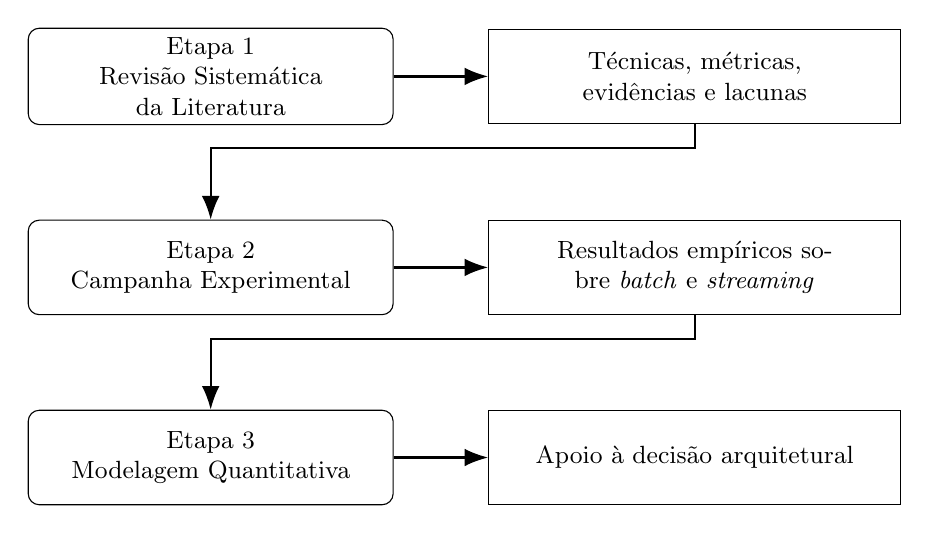
\begin{tikzpicture}[
node distance=1.2cm, 
etapa/.style={
rectangle,
rounded corners,
draw,
align=center,
text width=4.4cm,
minimum height=1.2cm,
font=\small
},
produto/.style={
rectangle,
draw,
align=center,
text width=5cm,
minimum height=1.2cm,
font=\small
},
seta/.style={-{Latex[length=3mm]}, thick}
]

\node[etapa] (rsl) {Etapa 1 \\ Revisão Sistemática da Literatura};
\node[produto, right=1.2cm of rsl] (rslout) {Técnicas, métricas, evidências e lacunas};

\node[etapa, below=of rsl] (exp) {Etapa 2 \\ Campanha Experimental};
\node[produto, right=1.2cm of exp] (expout) {Resultados empíricos sobre \textit{batch} e \textit{streaming}};

\node[etapa, below=of exp] (modelo) {Etapa 3 \\ Modelagem Quantitativa};
\node[produto, right=1.2cm of modelo] (modeloout) {Apoio à decisão arquitetural};


\draw[seta] (rsl) -- (rslout);
\draw[seta] (exp) -- (expout);
\draw[seta] (modelo) -- (modeloout);

\draw[seta] (rslout.south) -- ++(0,-0.3cm) -| (exp.north);
\draw[seta] (expout.south) -- ++(0,-0.3cm) -| (modelo.north);

\end{tikzpicture}
\caption{Desenho metodológico da pesquisa}
\label{fig:desenho-metodologico}
\end{figure}

A Revisão Sistemática da Literatura será detalhada no Capítulo~\ref{cap:rsl}, enquanto a campanha experimental será apresentada no Capítulo~\ref{cap:campanha-experimental}. Neste capítulo, o objetivo é apresentar a lógica metodológica geral que conecta essas etapas e justifica sua integração.

\section{Procedimentos de Análise}
\label{sec:procedimentos-analise}

A análise da Revisão Sistemática da Literatura foi conduzida em duas dimensões. A primeira dimensão foi qualitativa, envolvendo a leitura, classificação e categorização dos estudos primários. Essa análise permitiu identificar técnicas de \textit{design}, tipos de otimização, métricas utilizadas, estilos arquiteturais recorrentes e lacunas metodológicas. A segunda dimensão foi quantitativa e exploratória, utilizando o \textit{Log Response Ratio} (LRR) como medida normalizada de efeito. Essa escolha permitiu comparar estudos que utilizaram diferentes métricas de desempenho, como tempo de execução, latência, \textit{throughput} e \textit{speedup}.

A análise da campanha experimental foi conduzida a partir das métricas coletadas durante as execuções. Entre as métricas consideradas estão tempo total de execução, \textit{throughput}, latência, uso de CPU, consumo de memória, \textit{backpressure}, taxa de processamento e métricas de entrada e saída dos contêineres. Essas métricas permitiram avaliar o comportamento dos paradigmas \textit{batch} e \textit{streaming} sob diferentes volumes de dados, taxas de eventos, números de \textit{workers} e intervalos de \textit{trigger}.

Para verificar se as diferenças observadas entre cenários eram estatisticamente significativas, foram utilizados procedimentos estatísticos não paramétricos. Inicialmente, foi aplicado o teste de Shapiro-Wilk para avaliar a normalidade das distribuições das métricas coletadas \cite{shapiro1965analysis}. Considerando que distribuições de desempenho em sistemas computacionais nem sempre podem ser assumidas como normalmente distribuídas, foram utilizados testes não paramétricos nas comparações entre cenários.

Para comparações entre dois grupos independentes, foi aplicado o teste de Mann-Whitney U \cite{mann1947test}. Para comparações entre múltiplos grupos, foi utilizado o teste de Kruskal-Wallis \cite{kruskal1952use}. Quando identificadas diferenças significativas entre múltiplos cenários, foram aplicados testes \textit{pós-hoc} de Dunn com correção de Bonferroni \cite{dunn1964multiple}. Além dos testes de significância, foi utilizado o tamanho de efeito de Cliff's Delta para avaliar a magnitude das diferenças entre distribuições \cite{cliff1993dominance}.

A etapa de modelagem quantitativa será conduzida a partir da integração entre os achados da literatura, os resultados experimentais e características informacionais dos dados. A proposta não busca substituir a experimentação, mas oferecer uma forma de apoio preliminar à análise de alternativas arquiteturais. A intenção é investigar se características como volume, taxa de eventos, entropia, redundância e variabilidade podem ser relacionadas a métricas de desempenho, contribuindo para uma tomada de decisão arquitetural mais fundamentada.

\section{Validade da Pesquisa}
\label{sec:validade-pesquisa}

A validade da pesquisa será analisada considerando possíveis ameaças à validade interna, externa, de construção e de conclusão. Essa organização é comum em estudos experimentais em Engenharia de Software e contribui para tornar explícitas as limitações do desenho experimental, da coleta de dados e da interpretação dos resultados \cite{wohlin2012experimentation}.

A validade interna está relacionada à capacidade de atribuir os efeitos observados às variáveis controladas no experimento. Para mitigar ameaças internas, os cenários foram definidos previamente, as execuções foram automatizadas e as métricas foram coletadas de forma sistemática. Além disso, cada cenário foi executado repetidas vezes, reduzindo a influência de variações ocasionais do ambiente.

A validade externa refere-se à possibilidade de generalização dos resultados para outros contextos. Como o experimento utiliza um ambiente específico, baseado em Spark, Kafka e um \textit{dataset} definido, os resultados devem ser interpretados dentro desse contexto. A ampliação para outros \textit{datasets}, tecnologias e ambientes de execução será indicada como possibilidade de trabalhos futuros.

A validade de construção está relacionada à adequação das métricas utilizadas para representar os conceitos investigados. Para mitigar essa ameaça, foram utilizadas métricas amplamente adotadas em avaliações de desempenho, como \textit{throughput}, latência, uso de recursos, \textit{backpressure} e escalabilidade.

A validade de conclusão diz respeito à adequação dos procedimentos estatísticos utilizados para interpretar os resultados. Para reduzir essa ameaça, foram aplicados testes de normalidade, testes não paramétricos, pós-testes e medidas de tamanho de efeito, evitando conclusões baseadas apenas em médias ou observações visuais.

Dessa forma, a metodologia proposta permite que a pesquisa avance de uma compreensão ampla da literatura para uma avaliação empírica específica e, posteriormente, para uma proposta de modelagem quantitativa voltada ao apoio à decisão arquitetural em sistemas intensivos em dados.

\chapter{Revisão Sistemática da Literatura}
\label{cap:rsl}

A Revisão Sistemática da Literatura (RSL) constituiu a primeira etapa da pesquisa e teve como objetivo consolidar evidências empíricas sobre estratégias de \textit{design}, técnicas arquiteturais, métricas de avaliação e lacunas relacionadas a sistemas intensivos em dados. Essa etapa fornece a base conceitual e empírica para a campanha experimental e para a proposta de um modelo de apoio à decisão arquitetural.

A RSL resultou no artigo intitulado \textit{Design of Data-Intensive Systems: A Systematic Review with Exploratory Quantitative Synthesis}, submetido ao WEBIST 2026. No momento da elaboração desta proposta, o artigo encontra-se aguardando aprovação. Essa submissão representa um dos resultados parciais desta pesquisa e consolida a etapa de revisão sistemática desenvolvida no âmbito da dissertação.

A condução da revisão seguiu diretrizes reconhecidas para Revisões Sistemáticas da Literatura em Engenharia de Software \cite{kitchenham2007guidelines,kitchtchenham2009,kitchenham2015evidence} e utilizou o protocolo PRISMA 2020 como referência para relatar o processo de identificação, triagem, elegibilidade e inclusão dos estudos \cite{page2021prisma}. Além da síntese qualitativa, foi conduzida uma síntese quantitativa exploratória com o objetivo de comparar, de forma normalizada, os efeitos de diferentes otimizações arquiteturais reportadas na literatura.

\section{Objetivo e Questões de Pesquisa}
\label{sec:rsl-objetivo}

O objetivo da RSL foi identificar, organizar e sintetizar evidências sobre o \textit{design} de sistemas intensivos em dados, com ênfase em estratégias arquiteturais orientadas ao desempenho. A revisão buscou responder às seguintes questões de pesquisa:

\begin{enumerate}
    \item Quais técnicas e abordagens de \textit{design} são aplicadas em sistemas intensivos em dados?
    \item Quais métricas são utilizadas para avaliar o desempenho e a eficiência desses sistemas?
    \item Quais evidências quantitativas existem sobre a efetividade das diferentes abordagens?
    \item Quais estilos arquiteturais, \textit{frameworks} ou padrões de \textit{design} são mais recorrentes em sistemas intensivos em dados?
    \item Existem lacunas ou oportunidades para estudos futuros?
\end{enumerate}

Essas questões permitiram orientar a busca, a seleção, a extração dos dados e a análise dos estudos primários. A definição das questões também contribuiu para delimitar o foco da revisão, evitando a inclusão de estudos genéricos sobre \textit{Big Data} que não apresentassem relação direta com \textit{design} arquitetural, métricas de desempenho ou avaliação empírica.

\section{Estratégia de Busca}
\label{sec:rsl-estrategia-busca}

A busca foi realizada em quatro bibliotecas digitais: ACM Digital Library\footnote{\url{https://dl.acm.org/}}, IEEE Xplore\footnote{\url{https://ieeexplore.ieee.org}}, Scopus\footnote{\url{https://www.scopus.com}} e ScienceDirect\footnote{\url{https://www.sciencedirect.com/}}. Essas bases foram selecionadas por sua relevância para as áreas de Engenharia de Software, Sistemas Distribuídos, Arquitetura de Software e Computação Intensiva em Dados.

A estratégia de busca foi construída com base na estrutura PICO, considerando quatro dimensões principais: população, intervenção, comparação e resultado (\textit{outcome}). A população foi representada por termos associados a sistemas intensivos em dados, como \textit{data-intensive systems}, \textit{big data systems} e \textit{large-scale data systems}. A intervenção foi representada por termos relacionados a \textit{design}, arquitetura e projeto arquitetural. A comparação incluiu termos associados a atributos de qualidade, como desempenho, escalabilidade, confiabilidade e tolerância a falhas. O resultado foi representado por termos relacionados a métricas e avaliação quantitativa.

De forma geral, a \textit{string} de busca combinou os termos por meio de operadores booleanos, conforme a lógica apresentada a seguir:

\begin{equation}
S = (P) \land (I) \land (C) \land (O)
\label{eq:string-pico}
\end{equation}

em que $P$ representa os termos associados à população, $I$ representa os termos associados à intervenção, $C$ representa os termos associados aos atributos comparativos e $O$ representa os termos associados aos resultados esperados. Essa formulação permitiu estruturar a busca de modo sistemático e alinhado ao objetivo da revisão.

A busca foi conduzida em setembro de 2025. Foram considerados estudos publicados em periódicos revisados por pares ou em anais de conferências, desde que apresentassem relação direta com sistemas intensivos em dados, \textit{design} arquitetural, avaliação de desempenho ou otimizações sistêmicas.

\section{Critérios de Inclusão e Exclusão}
\label{sec:rsl-criterios}

Para assegurar a relevância e a qualidade dos estudos selecionados, foram definidos critérios de inclusão e exclusão antes da execução da triagem. Esses critérios foram aplicados nas etapas de leitura de títulos, resumos e textos completos.

\begin{table}[htbp]
\centering
\caption{Critérios de inclusão e exclusão da RSL}
\label{tab:criterios-rsl}
\footnotesize
\setlength{\tabcolsep}{6pt}
\renewcommand{\arraystretch}{1.3}
\begin{tabular}{p{6.2cm} p{6.2cm}}
\toprule
\textbf{Critérios de Inclusão} & \textbf{Critérios de Exclusão} \\ 
\midrule
Estudos publicados em periódicos revisados por pares ou conferências. & Estudos puramente conceituais, sem resultados empíricos. \\ 
Estudos sobre \textit{design}, arquitetura ou implementação de sistemas intensivos em dados. & Trabalhos sem métricas quantitativas ou sem descrição do ambiente experimental. \\ 
Trabalhos que comparam a solução proposta com pelo menos uma configuração de referência (\textit{baseline}). & Estudos não escritos em inglês. \\ 
Pesquisas com resultados quantitativos, como desempenho, escalabilidade ou consumo de recursos. & Trabalhos sobre sistemas de dados em geral, sem foco específico em sistemas intensivos em dados ou \textit{design} arquitetural. \\ 
Estudos com texto completo disponível e documentação mínima do ambiente experimental. & Revisões de literatura, meta-análises, cartas, editoriais ou capítulos de livro. \\ 
\bottomrule
\multicolumn{2}{l}{\footnotesize Fonte: elaborado pelo autor.}
\end{tabular}
\end{table}

Nos casos em que houve dúvidas sobre a aplicação dos critérios, a decisão foi discutida entre os revisores. Quando não foi possível alcançar consenso, um avaliador independente foi consultado. As razões de exclusão foram registradas ao longo do processo, garantindo maior transparência e rastreabilidade à revisão.

\section{Processo de Seleção dos Estudos}
\label{sec:rsl-selecao}

O processo de busca nas quatro bibliotecas digitais identificou 979 registros. A distribuição inicial foi de 448 artigos na ACM Digital Library, 215 na IEEE Xplore, 35 na ScienceDirect e 281 na Scopus. Após a remoção de 100 duplicatas, restaram 879 estudos únicos para a etapa de triagem.

A triagem por títulos e resumos resultou na exclusão de 600 registros que não atendiam aos critérios estabelecidos. Em seguida, 279 textos completos foram avaliados. Nessa etapa, 269 estudos foram excluídos, principalmente por não apresentarem resultados quantitativos compatíveis com o foco da síntese, por não descreverem adequadamente o ambiente experimental ou por não permitirem comparação com uma configuração de referência.

Ao final do processo, 10 estudos atenderam a todos os critérios de elegibilidade e qualidade, sendo incluídos tanto na Revisão Sistemática da Literatura quanto na síntese quantitativa exploratória.

A Figura~\ref{fig:prisma-rsl} apresenta o fluxo de seleção dos estudos de acordo com o modelo PRISMA 2020.

\begin{figure}[htbp]
\centering
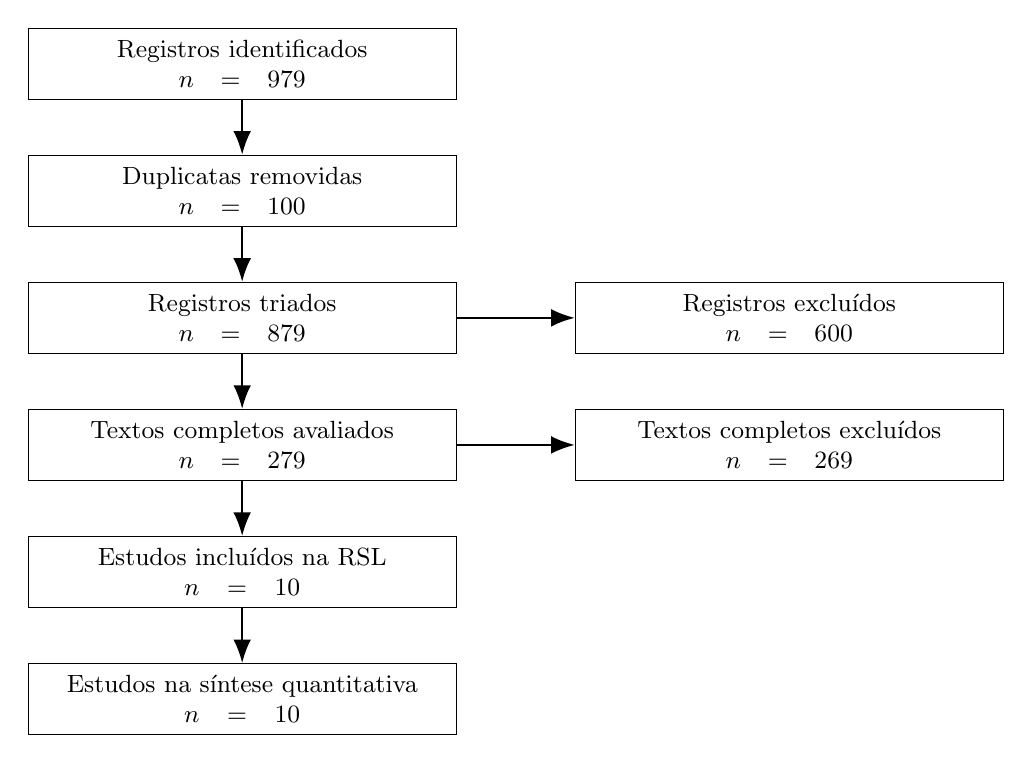
\begin{tikzpicture}[
node distance=0.7cm,
caixa/.style={
rectangle,
draw,
align=center,
text width=5.2cm,
minimum height=0.9cm,
font=\small
},
seta/.style={-{Latex[length=3mm]}, thick}
]
\node[caixa] (id) {Registros identificados \\ $n = 979$};
\node[caixa, below=of id] (dup) {Duplicatas removidas \\ $n = 100$};
\node[caixa, below=of dup] (triados) {Registros triados \\ $n = 879$};
\node[caixa, right=1.5cm of triados] (excluidos) {Registros excluídos \\ $n = 600$};
\node[caixa, below=of triados] (full) {Textos completos avaliados \\ $n = 279$};
\node[caixa, right=1.5cm of full] (fullex) {Textos completos excluídos \\ $n = 269$};
\node[caixa, below=of full] (incluidos) {Estudos incluídos na RSL \\ $n = 10$};
\node[caixa, below=of incluidos] (sintese) {Estudos na síntese quantitativa \\ $n = 10$};

\draw[seta] (id) -- (dup);
\draw[seta] (dup) -- (triados);
\draw[seta] (triados) -- (full);
\draw[seta] (full) -- (incluidos);
\draw[seta] (incluidos) -- (sintese);
\draw[seta] (triados) -- (excluidos);
\draw[seta] (full) -- (fullex);
\end{tikzpicture}
\caption{Fluxo PRISMA 2020 do processo de seleção dos estudos}
\label{fig:prisma-rsl}
\end{figure}

A Tabela~\ref{tab:distribuicao-bases} apresenta a distribuição dos registros identificados por base de dados.

\begin{table}[htbp]
\centering
\caption{Distribuição dos registros identificados por base de dados}
\label{tab:distribuicao-bases}
\small
\begin{tabular}{p{6cm} p{4cm}}
\toprule
\textbf{Base de dados} & \textbf{Registros identificados} \\ 
\midrule
ACM Digital Library & 448 \\ 
IEEE Xplore & 215 \\ 
ScienceDirect & 35 \\ 
Scopus & 281 \\ 
\midrule
\textbf{Total} & \textbf{979} \\ 
\bottomrule
\multicolumn{2}{l}{\footnotesize Fonte: elaborado pelo autor.}
\end{tabular}
\end{table}

\section{Avaliação da Qualidade}
\label{sec:rsl-qualidade}

A avaliação da qualidade dos estudos foi conduzida com base em um \textit{checklist} composto por 14 critérios. Esses critérios avaliaram aspectos como clareza do problema, aderência ao tema, descrição do contexto, metodologia, uso de dados experimentais, métricas arquiteturais, replicabilidade, limitações, recomendações práticas, apresentação de valores numéricos, comparabilidade das métricas, descrição do ambiente experimental, medidas de dispersão e comparação entre técnicas ou arquiteturas.

Cada critério recebeu uma das seguintes pontuações: Sim = 1, Parcialmente = 0,5 e Não = 0. Considerando os 14 critérios, a pontuação máxima possível para cada estudo foi de 14 pontos. Foi adotado um ponto de corte de 8 pontos, correspondente a aproximadamente 60\% da pontuação máxima, conforme representado pela Equação~\ref{eq:qa-score}.

\begin{equation}
QA_{min} = 0.60 \times 14 = 8.4 \approx 8
\label{eq:qa-score}
\end{equation}

Apenas estudos que atingiram ou superaram esse limiar foram mantidos no conjunto final. A adoção desse critério buscou garantir que os estudos incluídos apresentassem qualidade metodológica mínima para sustentar a síntese qualitativa e a síntese quantitativa exploratória.

\begin{table}[htbp]
\centering
\caption{Dimensões avaliadas no checklist de qualidade}
\label{tab:dimensoes-qualidade}
\small
\setlength{\tabcolsep}{6pt}
\renewcommand{\arraystretch}{1.3}
\begin{tabular}{p{4cm} p{8cm}}
\toprule
\textbf{Dimensão} & \textbf{Aspectos avaliados} \\ 
\midrule
Clareza do estudo & Definição do problema, objetivo e aderência ao \textit{design} de sistemas intensivos em dados. \\ 
Contexto experimental & Descrição do sistema, volume de dados, ambiente de execução, \textit{hardware}, \textit{software} e \textit{workload}. \\ 
Métricas e resultados & Uso de métricas quantitativas, apresentação de valores numéricos e comparabilidade dos resultados. \\ 
Rigor metodológico & Metodologia clara, replicabilidade, uso de \textit{baseline} e apresentação de limitações. \\ 
Relevância prática & Diretrizes, recomendações ou implicações para o \textit{design} de sistemas intensivos em dados. \\ 
\bottomrule
\multicolumn{2}{l}{\footnotesize Fonte: elaborado pelo autor.}
\end{tabular}
\end{table}

\section{Extração dos Dados}
\label{sec:rsl-extracao}

Os dados foram extraídos por meio de um formulário padronizado, implementado em uma planilha previamente definida. Para cada estudo incluído, foram registrados os seguintes campos: identificação do estudo, autores, ano de publicação, veículo de publicação, base digital, tipo de sistema investigado, domínio de aplicação, técnica arquitetural ou otimização proposta, métricas utilizadas e resultados quantitativos reportados.

Também foram extraídas informações relacionadas ao ambiente experimental, incluindo \textit{hardware}, \textit{software}, \textit{datasets}, \textit{workloads}, número de execuções, médias, desvios-padrão, variâncias e demais medidas estatísticas, quando disponíveis. A extração foi conduzida por um revisor principal e verificada por um segundo revisor. Divergências foram resolvidas por discussão e, quando necessário, por consulta a um terceiro avaliador.

Essa etapa foi essencial para permitir tanto a síntese qualitativa quanto a síntese quantitativa exploratória, uma vez que os estudos selecionados apresentavam métricas heterogêneas e diferentes formas de relato experimental.

\section{Síntese Quantitativa Exploratória}
\label{sec:rsl-sintese-quantitativa}

Em vez de realizar uma meta-análise inferencial formal, esta pesquisa adotou uma síntese quantitativa exploratória. Essa decisão foi motivada pela ausência sistemática de medidas de variância, desvio-padrão e tamanho amostral em grande parte dos estudos primários. Diante dessa limitação, a ponderação individual dos estudos e a modelagem formal de efeitos aleatórios não seriam estatisticamente defensáveis.

Para permitir comparações entre estudos que utilizaram métricas heterogêneas, foi adotada a Razão de Resposta Logarítmica, ou \textit{Log Response Ratio} (LRR), como medida normalizada de efeito. De forma geral, o LRR pode ser definido como:

\begin{equation}
LRR_i = \ln(RR_i)
\label{eq:lrr}
\end{equation}

em que $RR_i$ representa a razão de resposta do estudo $i$. Quando a métrica analisada indicava que valores maiores eram melhores, como \textit{throughput} ou \textit{speedup}, a razão foi calculada conforme a Equação~\ref{eq:rr-maior-melhor}.

\begin{equation}
RR_i = \frac{M_{tratamento}}{M_{baseline}}
\label{eq:rr-maior-melhor}
\end{equation}

Quando a métrica indicava que valores menores eram melhores, como tempo de execução, latência ou tempo de recuperação, a razão foi invertida, conforme a Equação~\ref{eq:rr-menor-melhor}.

\begin{equation}
RR_i = \frac{M_{baseline}}{M_{tratamento}}
\label{eq:rr-menor-melhor}
\end{equation}

A média não ponderada dos valores de LRR foi utilizada para estimar a magnitude geral dos efeitos observados:

\begin{equation}
\overline{LRR} = \frac{1}{k}\sum_{i=1}^{k} LRR_i
\label{eq:lrr-medio}
\end{equation}

em que $k$ representa o número de estudos incluídos na síntese quantitativa. Para facilitar a interpretação, o LRR médio também pode ser convertido novamente para a escala de razão de resposta:

\begin{equation}
RR_{medio} = e^{\overline{LRR}}
\label{eq:rr-medio}
\end{equation}

Como o valor médio observado foi $\overline{LRR} = 0.981$, a razão média de resposta foi aproximadamente:

\begin{equation}
RR_{medio} = e^{0.981} \approx 2.7
\label{eq:rr-resultado}
\end{equation}

Esse resultado indica que, de forma exploratória, as otimizações analisadas apresentaram impacto médio positivo no desempenho, com ganhos aproximados de $2,7$ vezes em relação às configurações de referência. No entanto, esse valor deve ser interpretado com cautela, pois a síntese não utiliza ponderação por variância ou tamanho amostral.

\section{Estudos Incluídos e Resultados}
\label{sec:rsl-estudos-incluidos}

Os dez estudos incluídos na síntese quantitativa exploratória investigam diferentes tipos de otimizações em sistemas intensivos em dados, abrangendo desde técnicas de escalonamento e compilação SQL até estratégias de armazenamento, processamento próximo aos dados e tolerância a falhas \cite{wang2018hard,aung2019coordinate,alquwaiee2022performance,ponce2019upgrading,li2022karst,vincon2020nkv,lyu2022fine,haynes2016pipegen,schiavio2020dynamic,gotze2018nvm-aware}.

A Tabela~\ref{tab:estudos-lrr} apresenta uma síntese dos estudos incluídos, suas otimizações principais, métricas utilizadas e valores de LRR.

\begin{table}[htbp]
\centering
\caption{Síntese dos estudos primários incluídos na RSL}
\label{tab:estudos-lrr}
\textfloatsep=10pt
\footnotesize
\setlength{\tabcolsep}{4pt}
\renewcommand{\arraystretch}{1.25}
\begin{tabular}{p{3.2cm} p{4.2cm} p{3.2cm} r}
\toprule
\textbf{Estudo} & \textbf{Otimização principal} & \textbf{Métrica analisada} & \textbf{LRR} \\ 
\midrule
Wang et al. (2018) & Escalonamento em Spark/YARN & Taxa de conclusão & 0,233 \\ 
Aung et al. (2019) & Tolerância a falhas com \textit{checkpoint} & Tempo de recuperação & 0,357 \\ 
AlQuwaiee et al. (2022) & Modelagem de desempenho em Spark & Tempo de execução & 0,511 \\ 
Ponce et al. (2019) & Integração entre HPC e \textit{Big Data} & \textit{Throughput} & 0,631 \\ 
Li et al. (2022) & Protocolo transacional escalável & \textit{Throughput} & 0,693 \\ 
Vin{\c{c}}on et al. (2020) & Processamento próximo aos dados & Desempenho & 0,993 \\ 
Lyu et al. (2022) & Gerenciamento fino de recursos & Latência/custo & 1,273 \\ 
Haynes et al. (2016) & Geração de \textit{pipelines} de dados & \textit{Speedup} & 1,335 \\ 
Schiavio et al. (2020) & Otimização dinâmica de compilação & \textit{Speedup} & 1,482 \\ 
G{\"o}tze et al. (2018) & Layout de armazenamento para NVM & Desempenho & 2,303 \\ 
\bottomrule
\multicolumn{4}{l}{\footnotesize Fonte: elaborado pelo autor.}
\end{tabular}
\end{table}

Os resultados indicam que as maiores magnitudes de efeito estão associadas a intervenções em baixo nível, especialmente aquelas relacionadas a armazenamento, movimentação de dados e execução de consultas. Em contraste, otimizações em camadas de controle, como escalonamento e tolerância a falhas, apresentaram ganhos mais moderados, embora ainda relevantes do ponto de vista arquitetural.

\section{Distribuição Temática dos Estudos}
\label{sec:rsl-distribuicao-tematica}

A análise dos estudos incluídos permitiu agrupá-los em três categorias temáticas principais: otimização de consultas e execução, otimização de hardware e armazenamento, e integração e conectividade. A primeira categoria correspondeu a 40\% dos estudos, enquanto as duas demais representaram 30\% cada.

A Figura~\ref{fig:distribuicao-tematica} apresenta a distribuição temática dos estudos incluídos.

\begin{figure}[htbp]
\centering
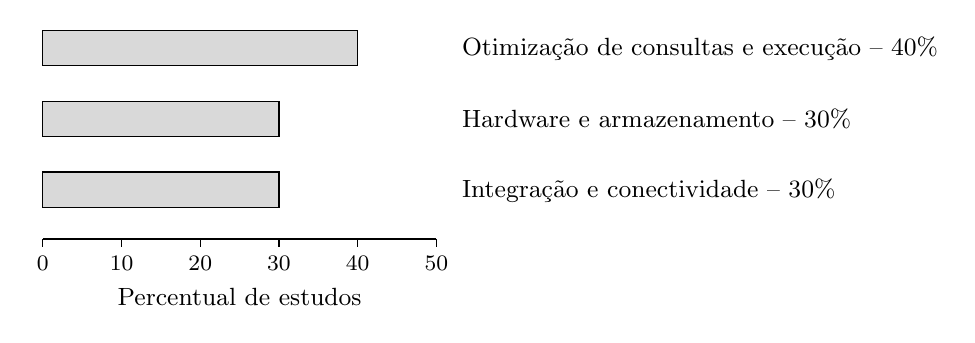
\begin{tikzpicture}

\draw[fill=gray!30] (0,1.4) rectangle (4,1.85);
\draw[fill=gray!30] (0,0.5) rectangle (3,0.95);
\draw[fill=gray!30] (0,-0.4) rectangle (3,0.05);


\node[anchor=west] at (5.2,1.62) {\small Otimização de consultas e execução -- 40\%};
\node[anchor=west] at (5.2,0.72) {\small Hardware e armazenamento -- 30\%};
\node[anchor=west] at (5.2,-0.18) {\small Integração e conectividade -- 30\%};


\draw[thick] (0,-0.8) -- (5,-0.8);

\foreach \x/\label in {0/0, 1/10, 2/20, 3/30, 4/40, 5/50} {
    \draw (\x,-0.8) -- (\x,-0.9);
    \node[anchor=north] at (\x,-0.9) {\footnotesize \label};
}
\node[anchor=north] at (2.5,-1.3) {\small Percentual de estudos};
\end{tikzpicture}
\caption{Distribuição temática dos estudos incluídos}
\label{fig:distribuicao-tematica}
\end{figure}

A categoria de otimização de consultas e execução inclui estudos relacionados ao escalonamento, à compilação SQL e ao gerenciamento de recursos. A categoria de hardware e armazenamento concentra estudos sobre memória não volátil, processamento próximo aos dados e protocolos transacionais escaláveis. A categoria de integração e conectividade reúne estudos voltados à eficiência na movimentação de dados, integração entre ambientes e tolerância a falhas.

Essa distribuição evidencia que parte significativa das contribuições da literatura está concentrada em camadas de execução e infraestrutura. Esse resultado reforça a importância de decisões arquiteturais que considerem não apenas a organização lógica do sistema, mas também aspectos de baixo nível, como armazenamento, movimentação de dados, execução de consultas e gerenciamento de recursos.

\section{Lacunas Identificadas}
\label{sec:rsl-lacunas}

A RSL permitiu identificar lacunas importantes na literatura sobre \textit{design} de sistemas intensivos em dados. A primeira lacuna refere-se à ausência de padronização no relato experimental. Muitos estudos reportam métricas como tempo de execução, latência, \textit{throughput} e \textit{speedup}, mas nem sempre apresentam informações suficientes sobre o número de execuções, medidas de dispersão, intervalos de confiança ou detalhes completos do ambiente experimental. Essa limitação dificulta a replicação dos estudos e restringe a realização de meta-análises inferenciais.

A segunda lacuna está relacionada à heterogeneidade das métricas e dos cenários avaliados. Embora os estudos investiguem sistemas intensivos em dados, as técnicas, \textit{workloads}, \textit{datasets}, ambientes e métricas variam significativamente. Essa diversidade reforça a necessidade de medidas normalizadas, como o LRR, mas também exige cautela na interpretação dos resultados agregados.

A terceira lacuna refere-se à concentração dos estudos em otimizações específicas. Muitos trabalhos analisam técnicas pontuais em ambientes controlados, mas poucos oferecem diretrizes gerais para apoiar decisões arquiteturais em contextos variados. Como consequência, ainda há necessidade de abordagens que auxiliem arquitetos de software a relacionar características dos dados, estratégias de processamento e métricas de desempenho.

A quarta lacuna envolve a limitada integração entre características dos dados e decisões arquiteturais. A maioria dos estudos avalia o desempenho a partir de métricas operacionais, mas poucos investigam como propriedades dos dados, como distribuição, cardinalidade, redundância, variabilidade ou entropia, podem influenciar a escolha entre alternativas arquiteturais. Essa lacuna sustenta a proposta desta dissertação de investigar uma abordagem quantitativa de apoio à decisão arquitetural baseada em evidências empíricas e características observáveis dos dados.

A partir dessas lacunas, a RSL fornece a base metodológica e empírica para as próximas etapas da pesquisa. Seus resultados justificam a condução da campanha experimental apresentada no Capítulo~\ref{cap:campanha-experimental} e fundamentam a proposta de um modelo quantitativo de apoio à decisão arquitetural em sistemas intensivos em dados.

\chapter{Campanha Experimental}
\label{cap:campanha-experimental}
 
A campanha experimental constituiu a segunda etapa da pesquisa e teve como objetivo avaliar empiricamente o comportamento de estratégias de processamento \textit{batch} e \textit{streaming} em um cenário de sistema intensivo em dados. Para isso, foi construído um ambiente experimental baseado em Apache Spark, Spark Structured Streaming, Apache Kafka e contêineres Docker, utilizando o \textit{dataset} NYC Taxi como fonte de dados.
 
A condução da campanha experimental foi motivada pelas lacunas identificadas na Revisão Sistemática da Literatura, especialmente a necessidade de evidências empíricas mais controladas, comparáveis e estatisticamente analisáveis. A partir dessa etapa, buscou-se observar como diferentes decisões arquiteturais e configurações operacionais afetam métricas como \textit{throughput}, latência, escalabilidade, consumo de recursos e estabilidade do processamento.
 
Nesta pesquisa, a campanha experimental é tratada como um experimento controlado principal, composto por múltiplos cenários experimentais. Essa organização permite avaliar diferentes fatores --- como volume de dados, taxa de eventos, número de \textit{workers} e intervalo de \textit{trigger} --- sem fragmentar a pesquisa em um conjunto de experimentos independentes. O desenho experimental foi orientado por princípios de experimentação em Engenharia de Software, considerando planejamento, definição de variáveis, controle de fatores, repetição das execuções e análise estatística dos resultados \cite{wohlin2012experimentation}.
 
\section{Objetivo e Questões Experimentais}
\label{sec:objetivo-questoes-experimento}
 
O objetivo da campanha experimental foi comparar, de forma empírica e reproduzível, o comportamento dos paradigmas de processamento \textit{batch} e \textit{streaming} sob diferentes condições de carga, paralelismo e configuração temporal. O foco recaiu sobre a análise de como decisões arquiteturais relacionadas ao paradigma de processamento, ao volume dos dados, à taxa de eventos, ao número de \textit{workers} e à cadência dos micro-lotes impactam o desempenho de um \textit{pipeline} intensivo em dados.
 
De modo geral, a campanha buscou responder à seguinte questão norteadora: \textit{como diferentes estratégias de processamento de dados se comportam em termos de throughput, latência, escalabilidade e consumo de recursos em um ambiente distribuído baseado em Spark e Kafka?}
 
A partir dessa questão geral, foram definidas quatro questões experimentais específicas:
 
\begin{enumerate}
    \item \textbf{RQ1:} Qual paradigma apresenta maior \textit{throughput} em sistemas intensivos em dados: processamento \textit{batch} ou processamento \textit{streaming}?
    \item \textbf{RQ2:} Como o volume de dados afeta o desempenho dos paradigmas \textit{batch} e \textit{streaming}?
    \item \textbf{RQ3:} Como a taxa de eventos e a cadência de micro-lotes afetam a latência e a estabilidade do processamento \textit{streaming}?
    \item \textbf{RQ4:} Como a escalabilidade horizontal afeta o desempenho dos paradigmas \textit{batch} e \textit{streaming}?
\end{enumerate}
 
A RQ1 compara diretamente os paradigmas de processamento. A RQ2 investiga o impacto do volume de dados sobre o desempenho de cada paradigma. A RQ3 analisa aspectos específicos do processamento em fluxo contínuo, especialmente a relação entre taxa de eventos e intervalo de \textit{trigger}. Por fim, a RQ4 investiga o efeito da escalabilidade horizontal --- medida pelo número de \textit{workers} Spark --- sobre o desempenho de ambos os paradigmas.
 
\section{Ambiente Experimental}
\label{sec:ambiente-experimental}
 
O ambiente experimental foi implementado utilizando contêineres Docker, com o objetivo de isolar e controlar os componentes do \textit{pipeline}. A arquitetura experimental incluiu um \textit{cluster} Spark, um serviço Kafka, \textit{scripts} de geração e envio de eventos, \textit{jobs} de processamento \textit{batch} e \textit{streaming}, além de \textit{scripts} de monitoramento e consolidação dos resultados. Todos os experimentos foram executados em uma máquina com processador AMD Ryzen 7 7435HS (8 núcleos físicos e 16 \textit{threads}), 61,53~GB de memória RAM, 467,35~GB de armazenamento interno e sistema operacional Linux (kernel 7.0.0-15-generic).
 
O Apache Spark foi utilizado como mecanismo de processamento distribuído. Nos cenários \textit{batch}, o Spark processou amostras de dados previamente armazenadas em disco. Nos cenários \textit{streaming}, o Spark Structured Streaming consumiu eventos publicados em tópicos Kafka e os processou continuamente por meio de micro-lotes \cite{armbrust2018structured,zaharia2016apache}.
 
O Apache Kafka atuou como sistema de mensageria distribuído e camada de ingestão dos eventos. Sua adoção permitiu simular um fluxo contínuo de dados, com produtores enviando registros em taxas controladas e consumidores processando os eventos por meio do Spark Structured Streaming \cite{kreps2011kafka}.
 
A Figura \ref{fig:arquitetura-experimento-vertical} apresenta uma visão geral da arquitetura experimental adotada.
 
\begin{figure}[htbp]
\centering
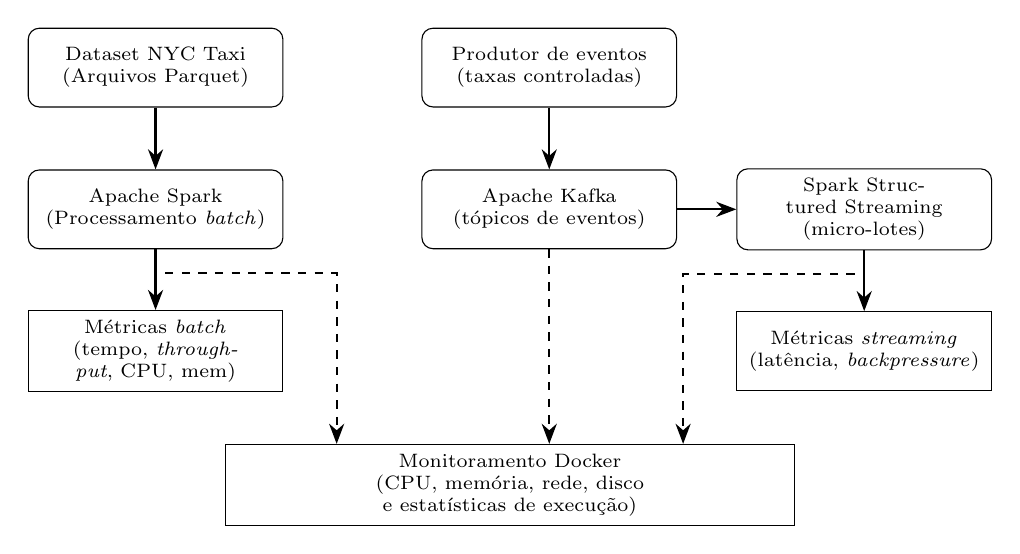
\begin{tikzpicture}[
    node distance=0.8cm and 0.4cm,
    bloco/.style={
        rectangle,
        rounded corners=4pt,
        draw=black,
        fill=white,
        align=center,
        text width=3.0cm,
        minimum height=1.0cm,
        font=\scriptsize
    },
    metrica/.style={
        rectangle,
        draw=black,
        fill=white,
        align=center,
        text width=3.0cm,
        minimum height=1.0cm,
        font=\scriptsize
    },
    monitor/.style={
        rectangle,
        draw=black,
        fill=white,
        align=center,
        text width=7.0cm,
        minimum height=1.0cm,
        font=\scriptsize
    },
    seta/.style={-{Stealth[scale=1.1]}, thick},
    coleta/.style={-{Stealth[scale=1.1]}, thick, dashed}
]
 
% CAMADA 1: INGESTÃO 
\node[bloco] (dados) at (0, 3.8) {Dataset NYC Taxi\\(Arquivos Parquet)};
\node[bloco] (produtor) at (5.0, 3.8) {Produtor de eventos\\(taxas controladas)};
 
% CAMADA 2: PROCESSAMENTO 
\node[bloco] (sparkbatch) at (0, 2.0) {Apache Spark\\(Processamento \textit{batch})};
\node[bloco] (kafka) at (5.0, 2.0) {Apache Kafka\\(tópicos de eventos)};
\node[bloco] (sparkstream) at (9.0, 2.0) {Spark Structured Streaming\\(micro-lotes)};
 
% CAMADA 3: RESULTADOS 
\node[metrica] (metricabatch) at (0, 0.2) {Métricas \textit{batch}\\(tempo, \textit{throughput}, CPU, mem)};
\node[metrica] (metricastream) at (9.0, 0.2) {Métricas \textit{streaming}\\(latência, \textit{backpressure})};

% CAMADA 4: MONITORAMENTO GLOBAL 
\node[monitor] (monitoramento) at (4.5, -1.5) {Monitoramento Docker\\(CPU, memória, rede, disco\\e estatísticas de execução)};
 
% --- CONEXÕES DO FLUXO BATCH (ESQUERDA) ---
\draw[seta] (dados) -- (sparkbatch);
\draw[seta] (sparkbatch) -- (metricabatch);
 
% --- CONEXÕES DO FLUXO STREAMING (DIREITA) ---
\draw[seta] (produtor) -- (kafka);
\draw[seta] (kafka) -- (sparkstream);
\draw[seta] (sparkstream) -- (metricastream);
 

\draw[coleta] (sparkbatch.south) -- ++(0,-0.3cm) -| ([xshift=-2.2cm]monitoramento.north);
\draw[coleta] (kafka.south) -- (kafka.south |- monitoramento.north);
\draw[coleta] (sparkstream.south) -- ++(0,-0.3cm) -| ([xshift=2.2cm]monitoramento.north);
 
\end{tikzpicture}
\caption{Arquitetura geral da campanha experimental organizada em camadas funcionais.}
\label{fig:arquitetura-experimento-vertical}
\end{figure}

A Figura \ref{fig:arquitetura-experimento-vertical} detalha a arquitetura em camadas adotada na campanha experimental, dividida em três pilares principais: ingestão, processamento e telemetria. Na camada superior, os dados históricos do Dataset NYC Taxi alimentam o ecossistema batch via Apache Spark, enquanto o Produtor de Eventos simula a chegada contínua de dados em tempo real com taxas controladas para o Apache Kafka. No núcleo do processamento, o Apache Spark manipula os dados em lote e o Spark Structured Streaming consome os tópicos do Kafka em micro-lotes, gerando as respectivas métricas de desempenho e resiliência (throughput, latência e backpressure). Por fim, integrado na base da infraestrutura, o módulo de Monitoramento Docker atua de forma transversal por meio de conexões de telemetria (representadas pelas linhas tracejadas), coletando continuamente o consumo de recursos físicos cruciais como CPU, memória, rede e disco durante a execução de ambos os fluxos.


\section{Dataset e Preparação dos Dados}
\label{sec:dataset-experimento}
 
O \textit{dataset} utilizado na campanha experimental foi o NYC Taxi, amplamente empregado em estudos envolvendo processamento de dados em larga escala, análise de mobilidade urbana e \textit{workloads} analíticos distribuídos. Os dados foram utilizados no formato Parquet e organizados em amostras de diferentes tamanhos, permitindo avaliar o impacto do volume sobre o desempenho dos cenários experimentais.
 
Foram consideradas quatro escalas de dados: 200~MB, 1~GB, 3~GB e 10~GB. A utilização de volumes distintos teve como objetivo verificar se o aumento do tamanho do \textit{dataset} impacta de maneira semelhante os paradigmas \textit{batch} e \textit{streaming}, bem como avaliar se \textit{workloads} maiores favorecem a amortização de \textit{overheads} distribuídos.
 
Nos cenários \textit{batch}, os arquivos Parquet foram lidos e processados diretamente pelo Spark a partir do sistema de arquivos local. Nos cenários \textit{streaming}, os dados foram convertidos em eventos discretos e enviados ao Kafka por meio de \textit{scripts} produtores, respeitando taxas de emissão previamente definidas. Essa estratégia permitiu simular um fluxo contínuo de dados e controlar a pressão exercida sobre o \textit{pipeline} de \textit{streaming}.
 

\section{Variáveis e Métricas}
\label{sec:variaveis-metricas}
 
A campanha experimental foi estruturada a partir de variáveis independentes e dependentes. As variáveis independentes representam os fatores controlados durante a execução dos cenários; as variáveis dependentes correspondem às métricas coletadas para avaliar o comportamento do sistema.
 
A Tabela~\ref{tab:variaveis-independentes} apresenta as variáveis independentes consideradas, com seus respectivos valores.
 
\begin{table}[htbp]
\centering
\caption{Variáveis independentes da campanha experimental}
\label{tab:variaveis-independentes}
\small
\setlength{\tabcolsep}{6pt}
\renewcommand{\arraystretch}{1.35}
\begin{tabular}{p{4.8cm} p{7.8cm}}
\toprule
\textbf{Variável independente} & \textbf{Valores considerados} \\
\midrule
Paradigma de processamento    & Processamento \textit{batch} e processamento \textit{streaming} \\
Volume de dados               & 200~MB, 1~GB, 3~GB e 10~GB \\
Taxa de eventos               & 200, 500, 1.000 e 2.000 eventos por segundo \\
Número de \textit{workers} Spark & 1, 2 e 4 \textit{workers} \\
Intervalo de \textit{trigger} & 1~s, 2~s e 5~s \\
\bottomrule
\multicolumn{2}{l}{\footnotesize Fonte: elaborado pelo autor.}
\end{tabular}
\end{table}
 
Essas variáveis representam decisões ou configurações arquiteturais relevantes em \textit{pipelines} de dados. A escolha do paradigma define a forma geral de processamento; o volume e a taxa de eventos representam características da carga de trabalho; o número de \textit{workers} define o nível de paralelismo disponível; e o intervalo de \textit{trigger} determina a cadência de formação dos micro-lotes no Spark Structured Streaming.
 
A Tabela~\ref{tab:metricas-experimento} apresenta as principais métricas coletadas durante a campanha.
 
\begin{table}[htbp]
\centering
\caption{Métricas avaliadas na campanha experimental}
\label{tab:metricas-experimento}
\small
\setlength{\tabcolsep}{6pt}
\renewcommand{\arraystretch}{1.35}
\begin{tabular}{p{4.8cm} p{7.8cm}}
\toprule
\textbf{Métrica} & \textbf{Descrição} \\
\midrule
Tempo total de execução  & Tempo decorrido entre o início e a conclusão do processamento em cada cenário. \\
\textit{Throughput}      & Quantidade de registros ou eventos processados por unidade de tempo. \\
Latência                 & Intervalo de tempo entre a chegada de um evento e a conclusão de seu processamento, especialmente relevante nos cenários \textit{streaming}. \\
Uso de CPU               & Utilização média e máxima da CPU nos contêineres durante a execução. \\
Consumo de memória       & Uso médio e máximo de memória nos contêineres. \\
\textit{Backpressure}    & Indicador de pressão no \textit{pipeline} quando a taxa de chegada dos eventos supera a capacidade de processamento. \\
Taxa de processamento    & Métrica do Spark Structured Streaming que expressa o número de registros processados por segundo em cada micro-lote. \\
Rede e disco             & Tráfego de entrada e saída dos contêineres durante a execução dos cenários. \\
\bottomrule
\multicolumn{2}{l}{\footnotesize Fonte: elaborado pelo autor.}
\end{tabular}
\end{table}
 
O \textit{throughput} foi utilizado como métrica primária para comparar a capacidade de processamento entre os cenários. Formalmente, essa grandeza é expressa pela Equação~\ref{eq:throughput}:
 
\begin{equation}
\text{\textit{Throughput}} = \frac{N_{\text{registros}}}{T_{\text{processamento}}}
\label{eq:throughput}
\end{equation}
 
\noindent em que $N_{\text{registros}}$ representa a quantidade de registros processados e $T_{\text{processamento}}$ o tempo total de processamento.
 
Nos cenários de \textit{streaming}, a latência foi interpretada como o intervalo de tempo entre a produção de um evento e a conclusão de seu processamento pelo Spark Structured Streaming. Essa relação é representada pela Equação~\ref{eq:latencia}:
 
\begin{equation}
\text{Latência} = T_{\text{processamento\_evento}} - T_{\text{chegada\_evento}}
\label{eq:latencia}
\end{equation}
 
\noindent em que $T_{\text{processamento\_evento}}$ é o instante de conclusão do processamento e $T_{\text{chegada\_evento}}$ é o instante de chegada do evento ao \textit{pipeline}.
 
Essas métricas foram selecionadas porque representam dimensões complementares do desempenho de sistemas intensivos em dados. Enquanto \textit{throughput} e latência expressam a capacidade de processamento e o tempo de resposta do sistema, as métricas de CPU, memória, rede e disco permitem quantificar o custo computacional associado a cada configuração experimental.
 
\section{Cenários Experimentais}
\label{sec:cenarios-experimentais}
 
Os cenários experimentais foram organizados em blocos temáticos, permitindo isolar diferentes fatores e observar seus efeitos individuais sobre o desempenho do sistema. Ao todo, foram definidos 35 cenários, sendo 16 relacionados ao processamento \textit{batch} e 19 ao processamento \textit{streaming}.
 
A Tabela~\ref{tab:cenarios-experimentais} apresenta a organização geral dos cenários, seus objetivos e configurações principais.
 
\begin{table}[htbp]
\centering
\caption{Organização dos cenários experimentais}
\label{tab:cenarios-experimentais}
\footnotesize
\setlength{\tabcolsep}{5pt}
\renewcommand{\arraystretch}{1.30}
\begin{tabular}{l p{3.8cm} p{6.0cm} r}
\toprule
\textbf{Grupo} & \textbf{Objetivo} & \textbf{Configurações principais} & \textbf{Qtd.} \\
\midrule
BL1--BL4  & Avaliar o impacto do volume em \textit{batch}           & 200~MB, 1~GB, 3~GB e 10~GB; 1 \textit{worker}                              & 4  \\
BS1--BS12 & Avaliar escalabilidade horizontal em \textit{batch}     & 1, 2 e 4 \textit{workers} para cada volume de dados                        & 12 \\
SL1--SL4  & Avaliar o impacto da taxa em \textit{streaming}         & 200, 500, 1.000 e 2.000 eventos/s; \textit{trigger} de 1~s; 1 \textit{worker} & 4  \\
SS1--SS12 & Avaliar escalabilidade horizontal em \textit{streaming} & 1, 2 e 4 \textit{workers} para cada taxa de eventos                        & 12 \\
ST1--ST3  & Avaliar sensibilidade ao \textit{trigger}               & 1.000 eventos/s; 1 \textit{worker}; \textit{triggers} de 1~s, 2~s e 5~s   & 3  \\
\midrule
\textbf{Total} & --- & --- & \textbf{35} \\
\bottomrule
\multicolumn{4}{l}{\footnotesize Fonte: elaborado pelo autor.}
\end{tabular}
\end{table}
 
Os cenários \textit{batch} foram organizados em dois blocos. O primeiro (BL1--BL4) avaliou o impacto do volume de dados com número fixo de \textit{workers}. O segundo (BS1--BS12) avaliou a escalabilidade horizontal, variando o número de \textit{workers} para cada volume de dados. Essa estrutura permitiu verificar se o aumento do paralelismo produz ganhos consistentes ou se introduz custos de coordenação que limitam a eficiência esperada.
 
Os cenários \textit{streaming} foram divididos em três blocos. O primeiro (SL1--SL4) avaliou o impacto da taxa de eventos com \textit{trigger} fixo e um único \textit{worker}. O segundo (SS1--SS12) avaliou a escalabilidade horizontal variando o número de \textit{workers}. O terceiro (ST1--ST3) avaliou a sensibilidade do \textit{pipeline} de \textit{streaming} a diferentes intervalos de \textit{trigger}. Essa estrutura possibilitou analisar tanto a capacidade de absorção de eventos quanto a estabilidade temporal do processamento em fluxo contínuo.
 

\section{Execução e Repetições}
\label{sec:execucao-repeticoes}
 
Cada cenário foi executado 30 vezes. Considerando os 35 cenários definidos, a campanha experimental totalizou 1.050 execuções, conforme indicado na Equação~\ref{eq:total-execucoes}:
 
\begin{equation}
N_{\text{execuções}} = 35 \times 30 = 1.050
\label{eq:total-execucoes}
\end{equation}
 
A repetição dos cenários teve como objetivo reduzir a influência de variações aleatórias do ambiente e permitir uma análise estatística mais robusta das métricas coletadas. Antes da campanha completa, foi realizada uma etapa de validação operacional com uma execução por cenário. Essa validação verificou o funcionamento correto de todos os componentes do \textit{pipeline}, incluindo a infraestrutura Docker, o Kafka, o Spark, o produtor de eventos, a coleta de métricas, a geração de arquivos CSV e a consolidação dos resultados.
 
Após a validação operacional, a campanha completa foi executada com coleta automatizada das métricas. Os dados brutos foram armazenados em arquivos CSV e posteriormente consolidados para análise estatística e geração de relatórios.
 

\section{Automação e Coleta de Métricas}
\label{sec:automacao-coleta}
 
A execução experimental foi integralmente automatizada por meio de \textit{scripts} responsáveis por preparar o ambiente, gerar amostras de dados, executar os \textit{jobs} de processamento, monitorar os contêineres e consolidar os resultados. A automação teve como objetivos reduzir interferências manuais, aumentar a reprodutibilidade e padronizar a coleta das métricas\footnote{Os \textit{scripts} de automação, os arquivos de configuração do Docker e os dados brutos coletados estão disponíveis publicamente em: \url{https://github.com/jbruno97/stream-batch-experiment}.}.
 
Os artefatos produzidos incluem resultados brutos das execuções \textit{batch} e \textit{streaming}, séries temporais de métricas dos contêineres, estatísticas de micro-lotes, sumários por cenário, gráficos e relatórios textuais. Esses artefatos permitiram analisar tanto o comportamento agregado dos cenários quanto variações específicas observadas durante a execução dos \textit{jobs}.
 
A coleta de métricas dos contêineres permitiu monitorar CPU, memória, rede e disco ao longo de toda a execução. Nos cenários de \textit{streaming}, foram coletadas adicionalmente métricas específicas do Spark Structured Streaming, como taxa de processamento por micro-lote, latência de \textit{trigger}, latência de eventos e \textit{backpressure}.
 

\section{Procedimento de Análise Estatística}
\label{sec:analise-estatistica-experimento}
 
A análise dos resultados foi conduzida em etapas sequenciais. Inicialmente, foram calculadas estatísticas descritivas por cenário, incluindo média, mediana, desvio padrão e coeficiente de variação. Em seguida, foi aplicado o teste de Shapiro-Wilk para avaliar a normalidade das distribuições \cite{shapiro1965analysis}.
 
Como métricas de desempenho em sistemas computacionais não devem ser assumidas como normalmente distribuídas, foram adotados testes estatísticos não paramétricos. Para a comparação entre os paradigmas \textit{batch} e \textit{streaming}, foi aplicado o teste de Mann-Whitney U \cite{mann1947test}. Para comparações entre múltiplos grupos --- como diferentes volumes, taxas de eventos, intervalos de \textit{trigger} e quantidades de \textit{workers} --- foi utilizado o teste de Kruskal-Wallis \cite{kruskal1952use}. Quando necessário, foram aplicados testes pós-hoc de Dunn com correção de Bonferroni \cite{dunn1964multiple}.
 
Além dos testes de significância, foi calculado o tamanho de efeito de Cliff's Delta para avaliar a magnitude das diferenças entre distribuições \cite{cliff1993dominance}. Essa análise permitiu interpretar não apenas a existência de diferenças estatisticamente significativas, mas também sua relevância prática no contexto experimental.
 
A organização em cenários temáticos, a execução com 30 repetições por cenário, a coleta automatizada de métricas e o uso de testes não paramétricos fornecem uma base empírica rigorosa para discutir os \textit{trade-offs} envolvidos na escolha entre estratégias de processamento em sistemas intensivos em dados. Os resultados obtidos a partir dessa campanha são discutidos nos capítulos seguintes, com ênfase no impacto das decisões arquiteturais sobre \textit{throughput}, latência, escalabilidade e estabilidade do processamento.

\chapter{Resultados Parciais}
\label{cap:resultados}

Os resultados parciais obtidos até o momento estão organizados em três blocos principais: os achados da Revisão Sistemática da Literatura (RSL), a síntese quantitativa exploratória dos estudos primários e os resultados da campanha experimental conduzida para comparar o processamento \textit{batch} e o processamento \textit{streaming}. Ao final, discutem-se as implicações desses resultados para a construção do modelo de apoio à decisão arquitetural.

Os resultados apresentados ainda devem ser interpretados como parciais, pois a pesquisa se encontra em estágio de desenvolvimento. No entanto, eles já permitem identificar tendências relevantes sobre o comportamento de sistemas intensivos em dados e sobre os fatores que influenciam decisões arquiteturais relacionadas a desempenho, escalabilidade, latência e estabilidade operacional.

\section{Resultados da Revisão Sistemática da Literatura}
\label{sec:resultados-rsl}

A Revisão Sistemática da Literatura identificou inicialmente 979 registros nas quatro bibliotecas digitais selecionadas. Após a remoção de 100 duplicatas, restaram 879 registros únicos para triagem. A etapa de triagem por título, resumo e palavras-chave resultou na exclusão de 600 estudos. Em seguida, 279 textos completos foram avaliados quanto aos critérios de elegibilidade.

Ao final do processo, 10 estudos primários atenderam aos critérios de inclusão, exclusão e avaliação de qualidade. Esses estudos foram incluídos na síntese qualitativa e na síntese quantitativa exploratória. A distribuição inicial dos registros por biblioteca digital foi de 448 artigos na \textit{ACM Digital Library}, 215 na \textit{IEEE Xplore}, 35 na \textit{ScienceDirect} e 281 na \textit{Scopus}.

Esses resultados indicam que o tema possui presença relevante em bibliotecas voltadas à Computação, especialmente \textit{ACM Digital Library}, \textit{IEEE Xplore} e \textit{Scopus}. Entretanto, o número final de estudos incluídos foi reduzido, evidenciando que poucos trabalhos atendiam simultaneamente aos critérios de foco arquitetural, presença de avaliação empírica, comparação com um cenário de referência (\textit{baseline}) e disponibilidade de dados quantitativos.

A análise qualitativa dos estudos primários permitiu agrupá-los em três categorias principais. A primeira categoria corresponde à otimização de consulta e execução, incluindo estudos relacionados a escalonamento, compilação SQL e gerenciamento de recursos em ambientes de Big Data \cite{wang2018hard,schiavio2020dynamic,lyu2022fine}. A segunda categoria envolve otimizações de armazenamento e \textit{hardware}, contemplando estudos sobre NVM, processamento próximo aos dados (\textit{near-data processing}) e arquiteturas escaláveis para ingestão transacional \cite{gotze2018nvm-aware,vincon2020nkv,li2022karst}. A terceira categoria reúne estudos sobre integração, conectividade e confiabilidade, incluindo transferência de dados entre sistemas, integração HPC-Big Data e mechanisms de \textit{checkpoint} em \textit{pipelines} baseados em Apache Kafka \cite{haynes2016pipegen,ponce2019upgrading,aung2019coordinate}.

Além dessas categorias, foi identificado um estudo voltado à modelagem e predição de desempenho em aplicações Spark-HBase, contribuindo diretamente para a discussão sobre mecanismos de apoio à configuração e tomada de decisão em sistemas de Big Data \cite{alquwaiee2022performance}.

A análise desses estudos mostra que os ganhos de desempenho em sistemas intensivos em dados podem ser obtidos por intervenções em diferentes camadas da arquitetura. Isso reforça a hipótese de que decisões arquiteturais não devem ser analisadas isoladamente, mas sim como parte de um conjunto de relações interdependentes entre dados, processamento, armazenamento, comunicação e recursos computacionais.

\section{Resultados da Síntese Quantitativa Exploratória}
\label{sec:resultados-sintese-quantitativa}

A síntese quantitativa exploratória teve como objetivo estimar a magnitude dos efeitos reportados pelos estudos primários. Para isso, foi utilizado o \textit{Log Response Ratio} (LRR) como medida normalizada de efeito. Essa escolha permitiu comparar resultados provenientes de diferentes métricas, como tempo de execução, latência, \textit{throughput} e \textit{speedup}.

De forma geral, os resultados indicaram efeitos positivos associados às técnicas avaliadas nos estudos primários. A síntese apontou que intervenções arquiteturais ou sistêmicas podem produzir melhorias relevantes de desempenho, especialmente quando atuam sobre gargalos de armazenamento, movimentação de dados, compilação de consultas e gerenciamento de recursos.

O valor médio da síntese exploratória foi de $\overline{\text{LRR}} = 0{,}981$, correspondente a uma razão média de resposta de aproximadamente $2{,}7\times$ em relação às configurações de referência. Esse resultado sugere que, nos estudos analisados, as otimizações arquiteturais produziram ganhos expressivos de desempenho. No entanto, essa interpretação deve ser feita com cautela, pois a síntese foi baseada em média não ponderada e não em uma meta-análise inferencial formal.

A principal limitação observada na síntese quantitativa foi a ausência recorrente de informações completas sobre tamanho amostral, medidas de dispersão, intervalos de confiança e variância. Essa limitação impediu a aplicação de modelos estatísticos mais robustos, como modelos de efeitos aleatórios ponderados. Por esse motivo, a síntese foi tratada em caráter exploratório, com o objetivo de identificar tendências gerais e ordens de magnitude dos efeitos relatados.

Esse resultado é relevante para esta pesquisa porque reforça uma das lacunas centrais identificadas: embora existam evidências de ganhos de desempenho em sistemas intensivos em dados, essas evidências ainda se mostram fragmentadas, heterogêneas e de difícil comparação direta. Portanto, permanece necessária uma abordagem que combine evidências da literatura, dados experimentais controlados e características observáveis dos dados para apoiar decisões arquiteturais.

\section{Resultados da Campanha Experimental}
\label{sec:resultados-experimento}

A segunda etapa da pesquisa consistiu em uma campanha experimental controlada para comparar o processamento \textit{batch} e o processamento \textit{streaming} utilizando Apache Spark, Spark Structured Streaming e Apache Kafka. Os resultados foram organizados e estruturados de acordo com as quatro questões de pesquisa experimentais definidas no estudo.

\subsection{RQ1 --- Paradigmas de Processamento e Vazão Máxima}
Na primeira questão experimental (RQ1), foi avaliado qual paradigma apresenta maior \textit{throughput} bruto em sistemas intensivos em dados. Os resultados demonstraram que o paradigma \textit{batch} (mensurado em milhões de linhas por segundo) apresentou vazão massivamente superior ao \textit{streaming} (mensurado em linhas por segundo) em todas as escalas de carga de trabalho testadas. 

Para validar a significância das diferenças encontradas sem pressupostos de normalidade distributiva, aplicou-se o teste não-paramétrico de Mann-Whitney U de cauda dupla, complementado pelo cálculo do tamanho de efeito através do Delta de Cliff ($\delta$). Conforme sumariado na Tabela~\ref{tab:rq1_throughput}, as divergências são estatisticamente significativas ($p < 0{,}001$) com efeito máximo ($\delta = 1{,}0$), indicando ausência prática de sobreposição entre as distribuições das amostras.

\begin{table}[htbp]
\centering
\caption{Comparação de throughput e testes de significância não-paramétricos (RQ1).}
\label{tab:rq1_throughput}
\small
\rowcolors{2}{white}{gray!5} 
\setlength{\tabcolsep}{6pt} 
\begin{tabularx}{\textwidth}{Xcccc}
\toprule
\textbf{Comparação} & \textbf{\shortstack{Batch Médio\\(M linhas/s)}} & \textbf{\shortstack{Stream Médio\\(linhas/s)}} & \textbf{Valor-$p$} & \textbf{\shortstack{Tamanho de\\Efeito ($\delta$)}} \\
\midrule
BL1 $\times$ SL1 (200MB) & 1,76  & 159,18  & $< 0{,}001$ & Grande (1,0) \\
BL2 $\times$ SL2 (1GB)   & 6,87  & 374,26  & $< 0{,}001$ & Grande (1,0) \\
BL3 $\times$ SL3 (3GB)   & 13,44 & 741,22  & $< 0{,}001$ & Grande (1,0) \\
BL4 $\times$ SL4 (10GB)  & 20,74 & 1274,14 & $< 0{,}001$ & Grande (1,0) \\
\bottomrule
\end{tabularx}
\vspace{0.3em}
\begin{flushleft}
\footnotesize Fonte: elaborado pelo autor.
\end{flushleft}
\end{table}

Esse comportamento discrepante é ilustrado graficamente na Figura~\ref{fig:rq1_dual_axis}, evidenciando que enquanto o paradigma \textit{batch} cresce em escala de milhões de registros processados por segundo, o \textit{streaming} é severamente limitado pelos gargalos inerentes da arquitetura de mensageria contínua. Os custos adicionais estão associados à sobrecarga (\textit{overhead}) de rede e serialização no recebimento contínuo do Apache Kafka, coordenação e controle temporal de micro-lotes mínimos (\textit{micro-batching}) e mecanismos internos de tolerância a falhas por \textit{checkpointing} incremental.

\begin{figure}[htbp]
\centering
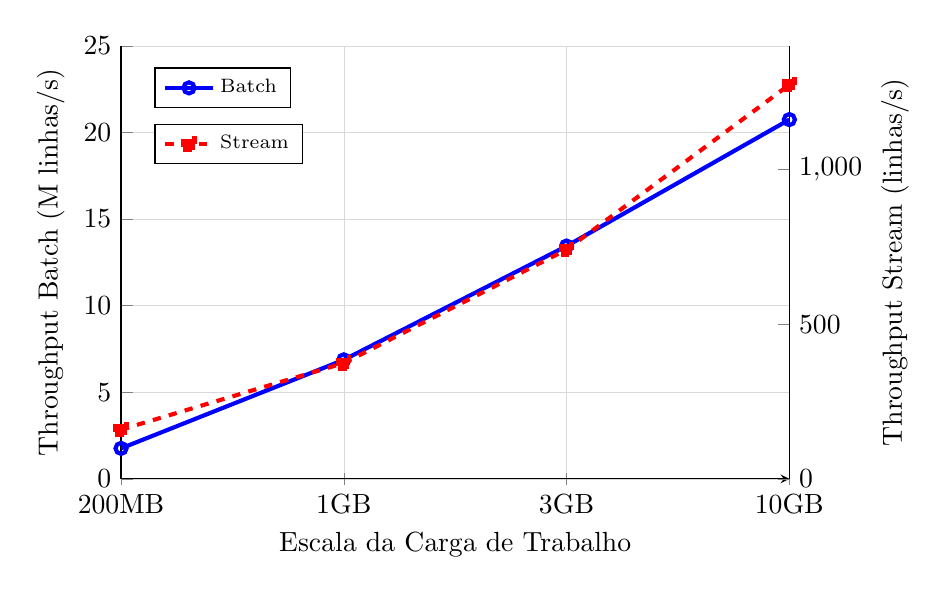
\begin{tikzpicture}

\begin{axis}[
    scale only axis,
    width=0.7\textwidth,
    height=5.5cm,
    xmin=0, xmax=3,
    xtick={0,1,2,3},
    xticklabels={200MB, 1GB, 3GB, 10GB},
    xlabel={Escala da Carga de Trabalho},
    ymin=0, ymax=25,
    ylabel={Throughput Batch (M linhas/s)},
    axis y line*=left,
    axis x line=bottom,
    grid=both,
    grid style={line width=.1pt, draw=gray!10},
    major grid style={line width=.2pt, draw=gray!30},
    legend style={at={(0.05,0.95)}, anchor=north west, font=\scriptsize}
]
\addplot[color=blue, mark=o, thick, line width=1.5pt] coordinates {
    (0, 1.76) (1, 6.87) (2, 13.44) (3, 20.74)
}; 
\addlegendentry{Batch}
\end{axis}

\begin{axis}[
    scale only axis,
    width=0.7\textwidth,
    height=5.5cm,
    xmin=0, xmax=3,
    ymin=0, ymax=1400,
    ylabel={Throughput Stream (linhas/s)},
    axis y line*=right,
    axis x line=none,
    xtick=\empty, 
    axis background/.style={fill=none}, 
    legend style={at={(0.05,0.82)}, anchor=north west, font=\scriptsize}
]
\addplot[color=red, mark=square*, dashed, thick, line width=1.5pt] coordinates {
    (0, 159.18) (1, 374.26) (2, 741.22) (3, 1274.14)
}; 
\addlegendentry{Stream}

\end{axis}
\end{tikzpicture}
\caption{Variações de throughput sob escalonamento de carga de trabalho (RQ1).}
\label{fig:rq1_dual_axis}
\end{figure}

Os resultados apresentados na Figura~\ref{fig:rq1_dual_axis} indicam comportamentos distintos entre os paradigmas analisados. Enquanto o processamento em \textit{batch} apresenta uma curva de crescimento acentuada conforme a carga aumenta, o modelo de \textit{stream} exibe estabilização precoce devido ao custo de coordenação das janelas de tempo. A análise estatística confirma que a diferença de desempenho observada é estatisticamente significativa ($p < 0{,}001$), validando a hipótese de que o dimensionamento da carga de trabalho afeta diretamente a eficiência das arquiteturas de processamento distribuído.


\subsection{RQ2 --- Impacto do Volume de Dados e Variabilidade Operacional}
Na segunda questão de pesquisa experimental (RQ2), investigou-se em que medida o escalonamento do volume de dados bruto afeta o desempenho interno e a estabilidade de cada paradigma de processamento. Para validar a significância estatística do impacto volumétrico sem assumir premissas de normalidade nas distribuições amostrais, aplicou-se o teste global não-paramétrico de Kruskal-Wallis. O teste confirmou com alto grau de confiança que o volume dos dados exerce um impacto estatisticamente significativo sobre a vazão operacional em ambos os cenários de arquitetura ($p < 0{,}001$).

Como o teste de Kruskal-Wallis aponta apenas a existência de diferença global, executaram-se análises \textit{post-hoc} utilizando o teste de comparações múltiplas de Dunn, aplicando a correção rígida de Bonferroni para mitigar a ocorrência de falsos positivos (erros do Tipo I). Os resultados dos testes par a par ratificaram que todas as transições de escala de dados (e.g., a passagem de 200MB para 1GB, e sucessivamente até 10GB) produzem variações de desempenho isoladamente significativas em ambos os ambientes computacionais.

A Tabela~\ref{tab:rq2_variance} expõe os resultados estruturados a partir do Coeficiente de Variação ($CV\%$), revelando o comportamento da dispersão relativa dos dados sob estresse volumétrico.

\begin{table}[htbp]
\centering
\caption{Análise de variabilidade operacional sob escalonamento volumétrico (RQ2).}
\label{tab:rq2_variance}
\small
\setlength{\tabcolsep}{6pt}
\begin{subtable}{0.48\linewidth}
\centering
\caption{Paradigma Batch}
\label{subtab:batch}
\begin{tabular}{lcc}
\toprule
\textbf{Cenário} & \textbf{Média (M linhas/s)} & \textbf{CV (\%)} \\
\midrule
BL1 (200MB) & 1,76  & 4,12 \\
BL2 (1GB)   & 6,87  & 2,85 \\
BL3 (3GB)   & 13,44 & 1,94 \\
BL4 (10GB)  & 20,74 & 1,10 \\
\bottomrule
\end{tabular}
\end{subtable}
\hfill
\begin{subtable}{0.48\linewidth}
\centering
\caption{Paradigma Stream}
\label{subtab:stream}
\begin{tabular}{lcc}
\toprule
\textbf{Cenário} & \textbf{Média (linhas/s)} & \textbf{CV (\%)} \\
\midrule
SL1 (200MB) & 159,18  & 8,45 \\
SL2 (1GB)   & 374,26  & 7,90 \\
SL3 (3GB)   & 741,22  & 9,12 \\
SL4 (10GB)  & 1274,14 & 11,34 \\
\bottomrule
\end{tabular}
\end{subtable}
\vspace{0.3em}
\begin{flushleft}
\footnotesize Fonte: elaborado pelo autor.
\end{flushleft}
\end{table}

A Figura~\ref{fig:rq2_variabilidade} ilustra o comportamento do Coeficiente de Variação frente ao aumento da carga de trabalho, permitindo contrastar visualmente a dinâmica de estabilização de ambos os paradigmas.

\begin{figure}[htbp]
\centering
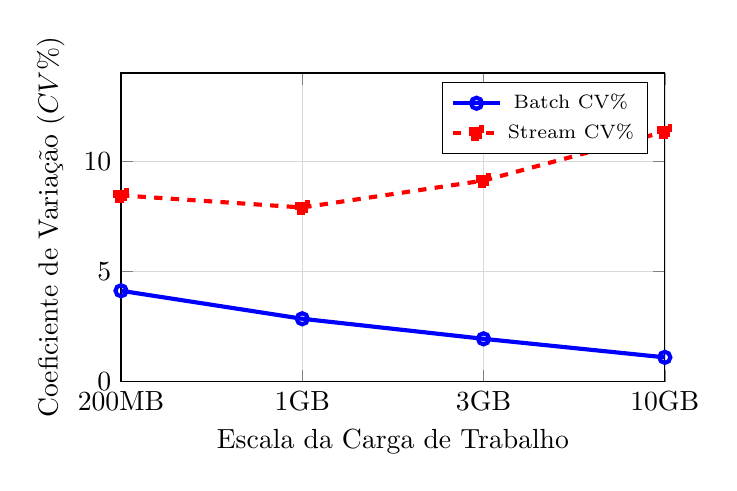
\begin{tikzpicture}
\begin{axis}[
    width=0.7\textwidth,
    height=5.5cm,
    xmin=0, xmax=3,
    xtick={0,1,2,3},
    xticklabels={200MB, 1GB, 3GB, 10GB},
    xlabel={Escala da Carga de Trabalho},
    ymin=0, ymax=14,
    ylabel={Coeficiente de Variação ($CV\%$)},
    grid=both,
    grid style={line width=.1pt, draw=gray!10},
    major grid style={line width=.2pt, draw=gray!30},
    legend pos=north east,
    legend style={font=\scriptsize}
]
% Linha do Batch
\addplot[color=blue, mark=o, thick, line width=1.5pt] coordinates {
    (0, 4.12) (1, 2.85) (2, 1.94) (3, 1.10)
}; \addlegendentry{Batch CV\%}

% Linha do Stream
\addplot[color=red, mark=square*, dashed, thick, line width=1.5pt] coordinates {
    (0, 8.45) (1, 7.90) (2, 9.12) (3, 11.34)
}; \addlegendentry{Stream CV\%}
\end{axis}
\end{tikzpicture}
\caption{Evolução da variabilidade operacional ($CV\%$) conforme a escala de carga (RQ2).}
\label{fig:rq2_variabilidade}
\end{figure}

A análise conjunta dos dados e do comportamento gráfico revela um fenômeno de divergência estrutural entre as duas abordagens arquiteturais. No paradigma \textit{batch}, constata-se que o aumento volumétrico atua como um fator de estabilização do cluster. À medida que a carga de dados cresce de 200MB para 10GB, o valor do $CV\%$ decresce de forma contínua, caindo de $4{,}12\%$ para meros $1{,}10\%$. 

Este comportamento é explicado pela amortização eficiente dos custos fixos computacionais em sistemas distribuídos. Cargas muito pequenas sofrem uma penalização proporcional elevada decorrente do \textit{overhead} de inicialização do ecossistema Spark, alocação de JVMs, registro de \textit{executors} e coordenação inicial do \textit{Task Scheduler}. Quando o volume de dados se torna massivo, o tempo gasto com o processamento real da carga domina a execução sobre os custos fixos de gerência, resultando em uma operação altamente previsível, estável e com baixa dispersão estatística.

Em contrapartida, o paradigma \textit{streaming} exibe uma curva de instabilidade ascendente. Embora ocorra uma leve oscilação positiva na transição inicial para 1GB ($7{,}90\%$), o avanço para volumes de 3GB e 10GB eleva o Coeficiente de Variação para $9{,}12\%$ e $11{,}34\%$, respectivamente. 

Este ganho de volatilidade indica que o escalonamento volumétrico em pipelines contínuos penaliza a consistência temporal da computação. Sob cargas elevadas, os nós do cluster enfrentam gargalos cumulativos na camada de rede (ingestão via tópicos do Apache Kafka), saturação de memória física durante as operações de agrupamento em micro-lotes e atrasos recorrentes na persistência dos metadados de \textit{checkpointing}. Essa disputa intensa por recursos computacionais gera picos localizados de latência e variações de processamento entre as janelas temporais, o que degrada a estabilidade macroscópica do sistema e eleva a incerteza operacional da arquitetura de fluxo contínuo.

\subsection{RQ3 --- Intervalos de Trigger e Latência de Eventos}
Na terceira questão de pesquisa experimental (RQ3), restringiu-se o escopo de análise ao ecossistema de processamento contínuo (\textit{streaming}) com o objetivo de mensurar as consequências operacionais da parametrização temporal dos gatilhos de execução (\textit{triggers}). Para determinar o impacto dessas variações de configuração, aplicou-se o teste não-paramétrico de Kruskal-Wallis. O modelo estatístico validou de forma robusta que a alteração programática do intervalo de \textit{trigger} resulta em modificações estatisticamente significativas nas métricas de latência e estabilidade do \textit{Spark Structured Streaming} ($p < 0{,}001$). 

A Tabela~\ref{tab:rq3_operational} consolida as variáveis de desempenho capturadas durante as sessões controladas sob os intervalos amostrais de $1\text{s}$, $2\text{s}$ e $5\text{s}$.

\begin{table}[htbp]
\centering
\caption{Métricas operacionais de streaming segmentadas por intervalo de trigger (RQ3).}
\label{tab:rq3_operational}
\small
\setlength{\tabcolsep}{5pt}
\begin{tabular}{lccccc}
\toprule
\textbf{Cenário} & \textbf{\shortstack{Lat. Trigger\\(ms)}} & \textbf{\shortstack{Lat. Evento\\(s)}} & \textbf{\shortstack{Backpressure\\(ms)}} & \textbf{\shortstack{Throughput\\(linhas/s)}} & \textbf{\shortstack{Jitter\\(ms)}} \\
\midrule
ST1 (1s) & 1464,70 & 1,42 & 240,10 & 745,20 & 75,90 \\
ST2 (2s) & 1828,00 & 2,15 & 115,40 & 742,10 & 122,90 \\
ST3 (5s) & 2571,00 & 5,60 & 42,80  & 739,80 & 152,60 \\
\bottomrule
\end{tabular}
\vspace{0.3em}
\begin{flushleft}
\footnotesize Fonte: elaborado pelo autor.
\end{flushleft}
\end{table}

A Figura~\ref{fig:rq3_tradeoff} ilustra graficamente o comportamento oposto da latência do evento em relação ao tempo de barramento reprimido (\textit{backpressure}), servindo como subsídio visual para o mapeamento de gargalos.

\begin{figure}[htbp]
\centering
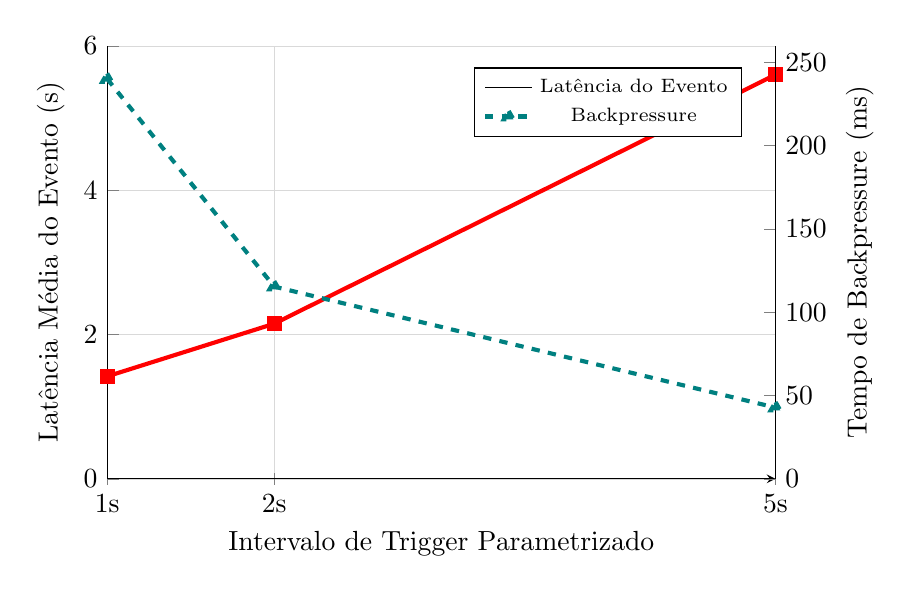
\begin{tikzpicture}
% CONFIGURAÇÃO DO PRIMEIRO EIXO (Esquerda - Latência do Evento)
\begin{axis}[
    scale only axis,
    width=0.7\textwidth,
    height=5.5cm,
    xmin=1, xmax=5,
    xtick={1,2,5},
    xticklabels={1s, 2s, 5s},
    xlabel={Intervalo de Trigger Parametrizado},
    ymin=0, ymax=6,
    ylabel={Latência Média do Evento (s)},
    axis y line*=left,
    axis x line=bottom,
    grid=both,
    grid style={line width=.1pt, draw=gray!10},
    major grid style={line width=.2pt, draw=gray!30}
]
\addplot[color=red, mark=square*, thick, line width=1.5pt] coordinates {
    (1, 1.42) (2, 2.15) (5, 5.60)
}; \label{plot:latencia}
\end{axis}

% CONFIGURAÇÃO DO SEGUNDO EIXO (Direita - Backpressure)
\begin{axis}[
    scale only axis,
    width=0.7\textwidth,
    height=5.5cm,
    xmin=1, xmax=5,
    ymin=0, ymax=260,
    ylabel={Tempo de Backpressure (ms)},
    axis y line*=right,
    axis x line=none,
    xtick=\empty,
    axis background/.style={fill=none}, 
    legend style={at={(0.95,0.95)}, anchor=north east, font=\scriptsize}
]

\addlegendimage{/pgfplots/refstyle=plot:latencia}\addlegendentry{Latência do Evento}

\addplot[color=teal, mark=triangle*, dashed, thick, line width=1.5pt] coordinates {
    (1, 240.10) (2, 115.40) (5, 42.80)
}; \addlegendentry{Backpressure}
\end{axis}
\end{tikzpicture}
\caption{Dilema arquitetural (trade-off) entre latência do evento e backpressure operacional (RQ3).}
\label{fig:rq3_tradeoff}
\end{figure}

Os dados empíricos e as curvas expostas revelam um \textit{trade-off} crítico de design arquitetural para engenharia de software de fluxos de dados. Observa-se que a dilatação deliberada do intervalo de gatilho de $1\text{s}$ para $5\text{s}$ atua de forma eficaz na mitigação da pressão imediata exercida sobre as filas de ingestão do sistema. Esse fenômeno é evidenciado pela redução drástica no tempo médio de interrupção por \textit{backpressure}, que cai de $240{,}10\text{ms}$ para meros $42{,}80\text{ms}$. Ao espaçar as execuções, o motor de micro-lotes ganha janelas mais folgadas para processar as mensagens retidas no Apache Kafka, reduzindo a concorrência imediata de escrita e o estresse sobre os buffers internos de memória do cluster.

Contudo, este alívio operacional impõe uma penalidade severa sobre os requisitos não-funcionais de reatividade e previsibilidade temporal do sistema. A latência média acumulada do evento sofre uma degradação expressiva, saltando de $1{,}42\text{s}$ para $5{,}60\text{s}$. Esse atraso é acompanhado por uma ampliação acentuada na instabilidade temporal da entrega dos dados (\textit{jitter}), que duplica de $75{,}90\text{ms}$ para $152{,}60\text{ms}$, sinalizando um comportamento de processamento altamente irregular e em rajadas (\textit{bursty}).

Adicionalmente, constata-se que a estratégia de acumular um volume maior de registros por ciclo (\textit{micro-batching} expandido) não se reverteu em ganhos de eficiência de vazão computacional, uma vez que o \textit{throughput} bruto permaneceu praticamente estagnado na faixa de 740 linhas por segundo em todos os cenários. Do ponto de vista de design de arquitetura de software, essa descoberta demonstra que a parametrização do \textit{trigger} não funciona como uma alavanca para o aumento de capacidade de vazão máxima, configurando-se estritamente como um botão de sintonia fina para equilibrar a tolerância a picos de carga contra a necessidade de processamento em tempo real estrito.

\subsection{RQ4 --- Escalabilidade Horizontal e Eficiência Arquitetural}
Na quarta questão de pesquisa (RQ4), avaliou-se a capacidade de resposta de ambos os paradigmas diante da expansão da infraestrutura computacional utilizando clusters com 1, 2 e 4 instâncias operacionais (\textit{workers}) sob a carga máxima de 10GB. Para quantificar a eficiência de paralelização, foram computadas as métricas de Speedup Observado ($S$) e Eficiência de Escalonamento ($E$), cujos resultados estão expostos na Tabela~\ref{tab:rq4_scalability_metrics}.

\begin{table}[htbp]
\centering
\caption{Métricas de escalabilidade e eficiência de paralelização no cluster (RQ4).}
\label{tab:rq4_scalability_metrics}
\small
\setlength{\tabcolsep}{6pt}
\begin{tabular}{lccccc}
\toprule
\textbf{Paradigma} & \textbf{Workers} & \textbf{Throughput Médio} & \textbf{Comportamento} & \textbf{Speedup ($S$)} & \textbf{Eficiência ($E$)} \\
\midrule
\textbf{Batch}   & 1 & 20,67 M linhas/s & Linha de Base  & 1,00 & 1,00 \\
                 & 2 & 29,67 M linhas/s & Sublinear      & 1,44 & 0,72 \\
                 & 4 & 30,92 M linhas/s & Saturação      & 1,50 & 0,38 \\
\midrule
\textbf{Stream}  & 1 & 1264,00 linhas/s & Linha de Base  & 1,00 & 1,00 \\
                 & 2 & 1220,00 linhas/s & Degradação     & 0,96 & 0,48 \\
                 & 4 & 1172,00 linhas/s & Ineficiência   & 0,93 & 0,23 \\
\bottomrule
\end{tabular}
\vspace{0.3em}
\begin{flushleft}
\footnotesize Fonte: elaborado pelo autor.
\end{flushleft}
\end{table}

A divergência estrutural entre as duas abordagens é evidente. O processamento \textit{batch} demonstra ganho positivo de escalabilidade horizontal ao expandir de 1 para 2 \textit{workers} ($S = 1{,}44$). Contudo, atinge um patamar de saturação precoce em 4 \textit{workers} ($S = 1{,}50$), onde a eficácia computacional cai para $38\%$, indicando que a sobrecarga distribuída de particionamento e coordenação passa a anular os benefícios do acréscimo de hardware.

No paradigma de \textit{streaming}, constata-se um cenário de escalabilidade negativa. A inserção de novos nós de processamento causou regressão no \textit{throughput} absoluto (reduzindo de 1264 para 1172 linhas/s em 4 \textit{workers}), derrubando a eficiência do cluster para pífios $23\%$. Esse comportamento deletério indica que a sobrecarga contínua associada à coordenação dos estágios, sincronização de \textit{offsets} no Apache Kafka e gestão de estado distribuído sob o modelo de micro-lotes impõe barreiras severas ao paralelismo horizontal. Esse fenômeno é mapeado comparativamente contra a linha ideal linear na Figura~\ref{fig:rq4_speedup_chart}.

\begin{figure}[htbp]
\centering
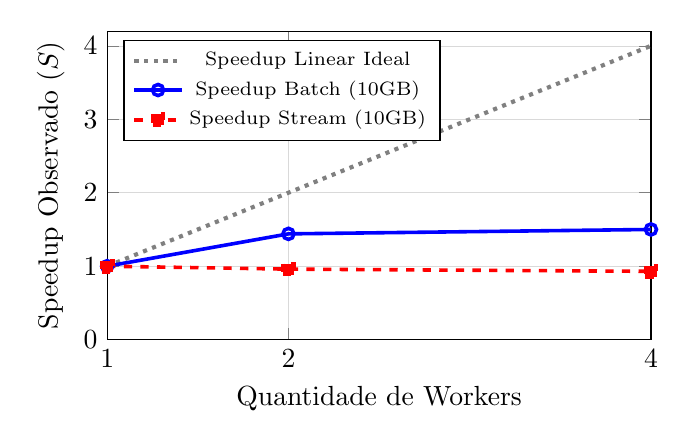
\begin{tikzpicture}
\begin{axis} [
    width=0.7\textwidth,
    height=5.5cm,
    xlabel={Quantidade de Workers},
    ylabel={Speedup Observado ($S$)},
    xmin=1, xmax=4,
    ymin=0, ymax=4.2,
    xtick={1,2,4},
    grid=both,
    grid style={line width=.1pt, draw=gray!10},
    major grid style={line width=.2pt, draw=gray!30},
    legend pos=north west,
    legend style={font=\scriptsize}
]
\addplot[color=gray, dotted, line width=1.5pt] coordinates {
    (1, 1) (2, 2) (4, 4)
}; \addlegendentry{Speedup Linear Ideal}

\addplot[color=blue, mark=o, thick, line width=1.3pt] coordinates {
    (1, 1.00) (2, 1.44) (4, 1.50)
}; \addlegendentry{Speedup Batch (10GB)}

\addplot[color=red, mark=square*, dashed, thick, line width=1.3pt] coordinates {
    (1, 1.00) (2, 0.96) (4, 0.93)
}; \addlegendentry{Speedup Stream (10GB)}
\end{axis}
\end{tikzpicture}
\caption{Curvas de speedup experimental frente ao limite linear ideal (RQ4).}
\label{fig:rq4_speedup_chart}
\end{figure}

A Tabela~\ref{tab:sintese-resultados-parciais} sintetiza as descobertas obtidas até o momento nas frentes de investigação mapeadas, servindo como base estrutural para a consolidação do modelo conceitual.

\begin{table}[htbp]
\centering
\caption{Síntese dos resultados parciais e implicações arquiteturais.}
\label{tab:sintese-resultados-parciais}
\scriptsize
\setlength{\tabcolsep}{4pt}
\renewcommand{\arraystretch}{1.3}
\begin{tabularx}{\textwidth}{lXX}
\toprule
\textbf{Dimensão Analisada} & \textbf{Resultado Parcial Consolidado} & \textbf{Implicação para o Modelo de Decisão} \\
\midrule
Revisão Sistemática & 10 estudos primários preencheram integralmente os critérios de elegibilidade e qualidade. & O volume reduzido evidencia a fragmentação de dados concretos para o design de sistemas intensivos em dados. \\
\midrule
Síntese Quantitativa & As otimizações arquiteturais exibiram efeito médio positivo ($\overline{\text{LRR}} = 0{,}981$), com razão de resposta de $\approx 2{,}7\times$. & Há indícios robustos de ganhos empíricos, mas as evidências na literatura carecem de padronização nos relatos estatísticos. \\
\midrule
RQ1 --- Batch vs Streaming & O paradigma \textit{batch} demonstrou superioridade de vazão em ordens de magnitude na comparação direta. & A escolha do paradigma deve priorizar os requisitos não-funcionais: maximização de throughput bruto (\textit{batch}) vs menor latência temporal (\textit{stream}). \\
\midrule
RQ2 --- Volume de Dados & O volume determinou a estabilização estatística do \textit{batch} ($CV = 1{,}10\%$) e o aumento de instabilidade do \textit{stream} ($CV = 11{,}34\%$). & O volume de dados bruto deve atuar como variável de entrada ponderada na matriz de decisão da arquitetura. \\
\midrule
RQ3 --- Triggers & O escalonamento do trigger (1s para 5s) mitigou o backpressure ($240\text{ms}$ para $42\text{ms}$), mas dobrou o jitter ($75\text{ms}$ para $152\text{ms}$). & Configurações de micro-lotes introduzem trade-offs matemáticos inevitáveis entre estabilidade temporal e vazão. \\
\midrule
RQ4 --- Escalabilidade & A adição de workers saturou o \textit{batch} ($E = 0{,}38$) e causou regressão de desempenho no \textit{streaming} ($E = 0{,}23$). & A infraestrutura horizontal não garante ganhos automáticos e depende da sensibilidade do paradigma ao overhead distribuído. \\
\bottomrule
\end{tabularx}
\vspace{0.3em}
\begin{flushleft}
\footnotesize Fonte: elaborado pelo autor.
\end{flushleft}
\end{table}

O mapeamento empírico consolidado na Tabela~\ref{tab:sintese-resultados-parciais} evidencia que a engenharia de sistemas intensivos em dados não pode se apoiar em premissas simplistas de escalonamento linear. Os comportamentos observados nas quatro questões de pesquisa demonstram que variáveis de infraestrutura (como a adição de \textit{workers}) e de configuração de \textit{runtime} (como intervalos de \textit{trigger}) desencadeiam reações severas e frequentemente contra-intuitivas na estabilidade e na vazão das arquiteturas distribuídas. A constatação de uma eficiência de paralelização decrescente no modelo \textit{batch} ($E = 0{,}38$) e abertamente regressiva no modelo de \textit{streaming} ($E = 0{,}23$) corrobora a necessidade de uma abordagem analítica formal para guiar decisões de design de software antes da alocação massiva de recursos computacionais.

Essa interdependência de fatores técnicos justifica a relevância de se unificar os achados empíricos em um arcabouço metodológico estruturado. Os dados de variabilidade da RQ2 e os \textit{trade-offs} temporais da RQ3 isolam os limiares operacionais onde cada paradigma deixa de ser eficiente. Consequentemente, essas métricas deixam de ser meros indicadores de desempenho passivos e passam a atuar como os parâmetros de entrada quantitativos indispensáveis para a calibração do modelo de decisão arquitetural proposto nesta pesquisa.


\section{Integração dos Resultados}
\label{sec:integracao-resultados}

Os resultados parciais da revisão sistemática e da campanha experimental convergem para uma mesma conclusão: decisões arquiteturais em sistemas intensivos em dados dependem fortemente do contexto. A literatura mostra que diferentes técnicas podem produzir ganhos relevantes, mas tais ganhos estão intrinsecamente associados a características específicas de \textit{workloads}, ambientes e métricas escolhidas. A campanha experimental, por sua vez, comprova que a escolha entre \textit{batch} e \textit{streaming}, bem como a configuração de paralelismo e \textit{trigger}, produz efeitos distintos sobre \textit{throughput}, latência, escalabilidade e estabilidade.

Essa convergência sustenta a necessidade de uma abordagem de apoio à decisão arquitetural. Em vez de assumir que uma técnica ou paradigma é universalmente superior, a decisão deve ponderar as características dos dados, os requisitos de desempenho e as restrições operacionais do sistema.

A principal contribuição dos resultados parciais reside na identificação de relações entre fatores arquiteturais e métricas observáveis. A Revisão Sistemática da Literatura indica que ganhos de desempenho podem ser obtidos em diferentes camadas do sistema. A campanha experimental demonstra que decisões como escolha do paradigma, variação do volume, ajuste de \textit{trigger} e aumento do número de \textit{workers} geram efeitos discrepantes dependendo do contexto operacional.



\section{Implicações para o Modelo de Apoio à Decisão}
\label{sec:implicacoes-modelo}

Os resultados obtidos até o momento fornecem insumos fundamentais para a especificação do modelo proposto. A Revisão Sistemática da Literatura indica quais tipos de decisões arquiteturais têm sido formalmente investigadas e quais métricas são adotadas para avaliá-las. A campanha experimental fornece evidências controladas sobre como fatores como volume, taxa de eventos, paralelismo e intervalo de \textit{trigger} degradam ou otimizam o comportamento de um \textit{pipeline} baseado em Apache Spark e Apache Kafka.

Esses resultados sugerem que o modelo de apoio à decisão deve incorporar múltiplas dimensões, destacando-se:
\begin{itemize}
    \item \textbf{Características dos dados:} tais como volume, distribuição, redundância e entropia;
    \item \textbf{Características da carga:} como taxa de eventos e variabilidade temporal;
    \item \textbf{Requisitos arquiteturais:} incluindo latência máxima aceitável e \textit{throughput} mínimo esperado;
    \item \textbf{Configurações operacionais:} como número de \textit{workers} e intervalo de \textit{trigger};
    \item \textbf{Métricas de custo computacional:} tais como perfil de uso de CPU, memória, rede e operações de disco.
\end{itemize}

Dessa forma, os resultados parciais não apenas respondem às questões iniciais da revisão e da campanha experimental, mas auxiliam na delimitação dos elementos que deverão compor a próxima etapa metodológica da pesquisa. Esses achados reforçam a necessidade de uma abordagem de apoio à decisão arquitetural que considere evidências empíricas, características intrínsecas dos dados e requisitos de desempenho, avançando além de recomendações genéricas ou dependentes exclusivamente da intuição do arquiteto de software.

\chapter{Cronograma}
\label{cap:cronograma}

O cronograma previsto para a continuidade da pesquisa estende-se até a defesa da dissertação, prevista para julho de 2027. O planejamento considera que parte das etapas iniciais da pesquisa já foi desenvolvida, incluindo a Revisão Sistemática da Literatura, a submissão de artigo derivado dessa etapa e a condução preliminar da campanha experimental.

As atividades restantes concentram-se no refinamento dos resultados experimentais, no aprofundamento da análise estatística, no cálculo de características informacionais dos dados, na construção do modelo quantitativo de apoio à decisão arquitetural, na validação preliminar da abordagem e na redação final da dissertação.


\begin{figure}[htbp]
\centering
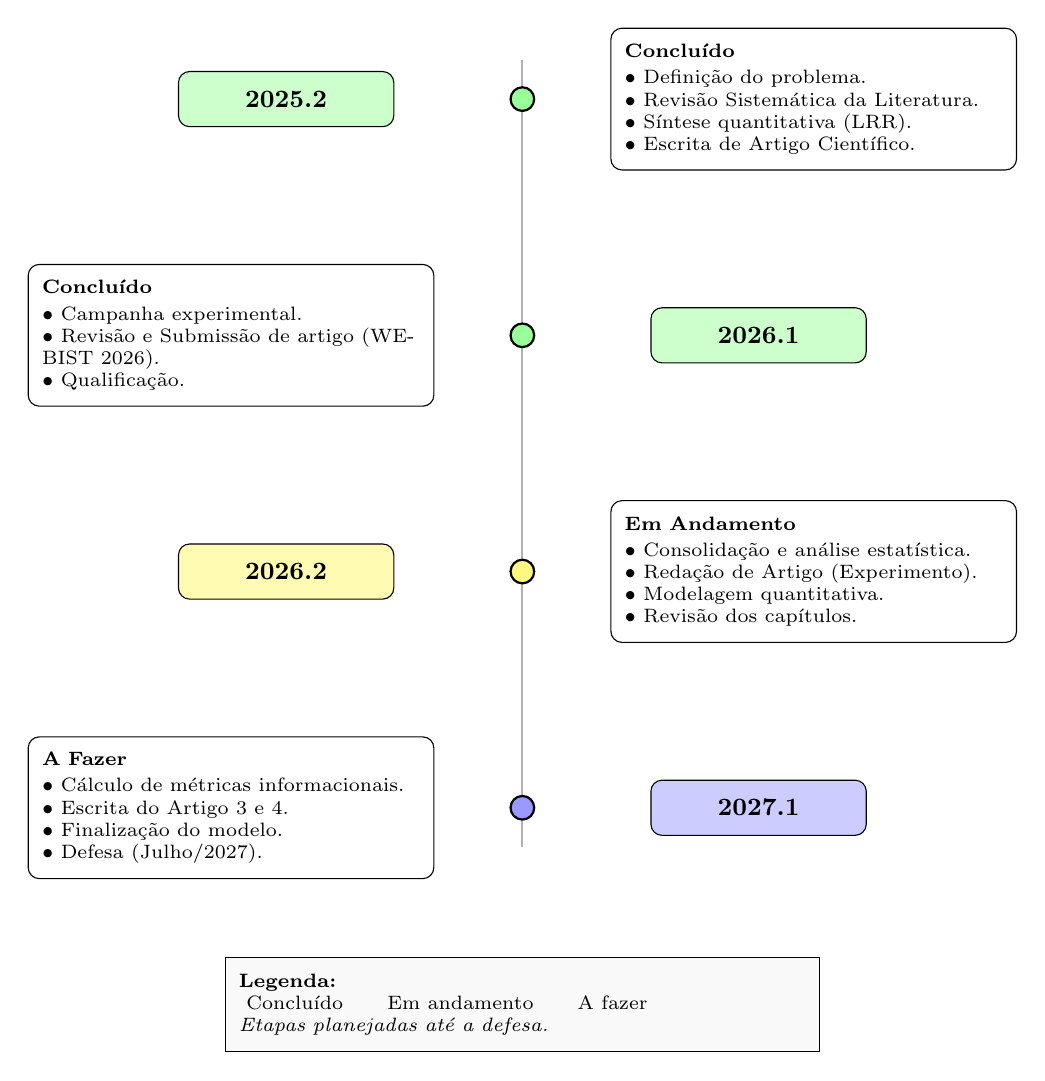
\begin{tikzpicture}[
    periodo/.style={
        rectangle, rounded corners, draw=black, align=center,
        text width=2.5cm, minimum height=0.7cm,
        font=\small\bfseries
    },
    atividade/.style={
        rectangle, rounded corners, draw=black, align=left,
        text width=4.8cm, minimum height=1.8cm,
        font=\scriptsize, fill=white, inner sep=5pt
    },
    legenda/.style={
        rectangle, draw=black, align=left,
        text width=7.2cm, minimum height=1.2cm,
        font=\scriptsize, fill=gray!5, inner sep=5pt
    }
]
% Linha central
\draw[thick, gray!60] (0,0.5) -- (0,-9.5);

% Períodos
\node[periodo, fill=green!20] at (-3,0) {2025.2};
\filldraw[fill=green!40, draw=black, thick] (0,0) circle (0.15);

\node[periodo, fill=green!20] at (3, -3) {2026.1};
\filldraw[fill=green!40, draw=black, thick] (0,-3) circle (0.15);

\node[periodo, fill=yellow!30] at (-3, -6) {2026.2};
\filldraw[fill=yellow!50, draw=black, thick] (0,-6) circle (0.15);

\node[periodo, fill=blue!20] at (3, -9) {2027.1};
\filldraw[fill=blue!40, draw=black, thick] (0,-9) circle (0.15);

% Atividades
\node[atividade] at (3.7,0) {
    \textbf{Concluído}\\[0.5ex]
    $\bullet$ Definição do problema.\\
    $\bullet$ Revisão Sistemática da Literatura.\\
    $\bullet$ Síntese quantitativa (LRR).\\
    $\bullet$ Escrita de Artigo Científico.
};

\node[atividade] at (-3.7, -3) {
    \textbf{Concluído}\\[0.5ex]
    $\bullet$ Campanha experimental.\\
    $\bullet$ Revisão e Submissão de artigo (WEBIST 2026).\\
    $\bullet$ Qualificação.
};

\node[atividade] at (3.7, -6) {
    \textbf{Em Andamento}\\[0.5ex]
    $\bullet$ Consolidação e análise estatística.\\
    $\bullet$ Redação de Artigo (Experimento).\\
    $\bullet$ Modelagem quantitativa.\\
    $\bullet$ Revisão dos capítulos.
};

\node[atividade] at (-3.7, -9) {
    \textbf{A Fazer}\\[0.5ex]
    $\bullet$ Cálculo de métricas informacionais.\\
    $\bullet$ Escrita do Artigo 3 e 4.\\
    $\bullet$ Finalização do modelo.\\
    $\bullet$ Defesa (Julho/2027).
};

% Legenda corrigida (Sem \tikz aninhado)
\node[legenda] at (0,-11.5) {
    \textbf{Legenda:}\\
    $\square$ Concluído \hspace{1em} $\square$ Em andamento \hspace{1em} $\square$ A fazer\\
    \textit{Etapas planejadas até a defesa.}
};
\end{tikzpicture}
\caption{Cronograma das atividades de pesquisa.}
\label{fig:cronograma-visual}
\end{figure}

\chapter{Próximos Passos}
\label{cap:proximos-passos}
Esta pesquisa já possui três componentes principais desenvolvidos: a Revisão Sistemática da Literatura (RSL) e a campanha experimental comparando processamento \textit{batch} e \textit{streaming}; ou em desenvolvimento: a verificação de condução de mais experimentos na campanha inicial e a formulação inicial de uma abordagem quantitativa de apoio à decisão arquitetural. Os próximos passos concentram-se no refinamento dessa abordagem, no cálculo de características informacionais dos dados, na integração destas aos resultados experimentais e na validação preliminar do modelo.

\section{Atividades Necessárias para a Conclusão da Pesquisa}
\label{sec:atividades-conclusao}
Os próximos passos da pesquisa estão relacionados à transformação dos resultados já obtidos em uma contribuição integrada. A intenção é que a dissertação apresente uma abordagem articulada de apoio à tomada de decisão arquitetural em sistemas intensivos em dados. As atividades previstas são apresentadas na Tabela~\ref{tab:proximos-passos}.

\begin{table}[htbp]
\centering
\caption{Atividades previstas para a continuidade da pesquisa.}
\label{tab:proximos-passos}
\small
\begin{tabular}{p{4cm} p{5.5cm} p{4cm}}
\toprule
\textbf{Atividade} & \textbf{Descrição} & \textbf{Resultado esperado} \\
\midrule
Consolidação experimental & Organizar tabelas, gráficos e resultados estatísticos. & Base de dados consolidada. \\
Cálculo de métricas informacionais & Calcular entropia, redundância, cardinalidade e variabilidade. & Caracterização informacional. \\
Refinamento do modelo & Definir entradas, saídas e critérios de ranqueamento. & Modelo quantitativo inicial. \\
Integração de resultados & Relacionar dados com métricas de desempenho. & Evidências de suporte. \\
Validação preliminar & Comparar recomendações com resultados observados. & Avaliação de coerência. \\
Redação final & Consolidar capítulos, revisar escrita e normas. & Versão final para defesa. \\
\bottomrule
\end{tabular}\vspace{0.3em}
\begin{flushleft}
\footnotesize Fonte: elaborado pelo autor.
\end{flushleft}\end{table}

\section{Refinamento do Modelo de Apoio à Decisão Arquitetural}
\label{sec:refinamento-modelo-proximos}
O modelo deverá considerar características associadas aos dados e ao processamento, como volume, taxa de eventos, entropia, redundância, cardinalidade, variabilidade, \textit{throughput}, latência e \textit{backpressure}. Um cenário de processamento é representado pelo vetor de características:
\begin{equation}
C_D = \{V, \lambda, H, R, K, \sigma, L_{req}\}
\label{eq:vetor-cenario-proximos}
\end{equation}
em que $V$ é o volume, $\lambda$ a taxa de eventos, $H$ a entropia, $R$ a redundância, $K$ a cardinalidade, $\sigma$ a variabilidade e $L_{req}$ a restrição de latência. Para cada alternativa arquitetural $a$, associa-se o conjunto de métricas $P_a = \{T_a, L_a, U_{cpu,a}, U_{mem,a}, B_a, E_a\}$. De forma exploratória, o escore de uma alternativa pode ser representado por:
\begin{equation}
S(a) = w_1T'_a + w_2L'_a + w_3U'_a + w_4E'_a
\label{eq:score-proximos}
\end{equation}
Essa formulação será refinada conforme a análise dos dados experimentais e a definição das métricas mais relevantes.

\section{Cálculo das Características Informacionais dos Dados}
\label{sec:calculo-caracteristicas-proximos}
Utilizando a Teoria da Informação, serão calculadas métricas como a entropia de Shannon:
\begin{equation}
H(X) = - \sum_{i=1}^{n} p(x_i) \log_2 p(x_i)
\end{equation}
e a redundância:
\begin{equation}
R(X) = 1 - \frac{H(X)}{H_{max}(X)}
\end{equation}
Essas métricas serão analisadas em conjunto com os dados experimentais, buscando correlações entre a estrutura da informação e o comportamento das arquiteturas sob carga.

\section{Produção Científica Prevista}
\label{sec:producao-cientifica-proximos}
Além da dissertação, a pesquisa prevê a produção de artigos conforme a Tabela~\ref{tab:producao-cientifica}.

\begin{table}[htbp]
\centering
\caption{Produção científica prevista.}
\label{tab:producao-cientifica}
\small
\begin{tabular}{llll}
\toprule
\textbf{Artigo} & \textbf{Tema} & \textbf{Situação} & \textbf{Período} \\
\midrule
Artigo 1 & RSL e Design de Sistemas & Submetido (WEBIST) & 2026.1 \\
Artigo 2 & Campanha Experimental & Em elaboração & 2026.2 \\
Artigo 3 & Modelo de Decisão & Planejado & 2026.2--2027.1 \\
Artigo 4 & Consolidação e Validação & Planejado & 2027.1 \\
\bottomrule
\end{tabular}
\vspace{0.3em}
\begin{flushleft}
\footnotesize Fonte: elaborado pelo autor.
\end{flushleft}
\end{table}

\section{Delimitação do Escopo e Trabalhos Futuros}
\label{sec:escopo-trabalhos-futuros}
O escopo está delimitado ao uso da RSL, da campanha experimental já conduzida e da validação preliminar do modelo. Trabalhos futuros poderão ampliar a pesquisa através da:
\begin{itemize}
    \item Avaliação com outros \textit{datasets} e tecnologias (e.g., Flink, Kafka Streams);
    \item Inclusão de métricas de custo financeiro, consumo energético e resiliência;
    \item Validação em ambientes de produção real;
    \item Desenvolvimento de ferramenta de automação para recomendações arquiteturais.
\end{itemize}



\phantompart
\bibliography{Bibliografia}

%%%%%%%%%%%%%%%%%%%%%%%%%%%%%%%%%%%%%%%%%%%%%%%%%%%%%%%%%%%%%%%%%%%%%%%%%%
% ELEMENTOS POS-TEXTUAIS
%%%%%%%%%%%%%%%%%%%%%%%%%%%%%%%%%%%%%%%%%%%%%%%%%%%%%%%%%%%%%%%%%%%%%%%%%%

\postextual

\renewcommand{\chapnumfont}{\chaptitlefont}
\renewcommand{\afterchapternum}{}
%\begin{apendicesenv}
\partapendices

\chapter{Material Complementar}

Inclua aqui materiais elaborados pelo autor que complementam a dissertacao.

\end{apendicesenv}

%\begin{anexosenv}
\partanexos

\chapter{Documento Complementar}

Inclua aqui materiais externos que complementam a dissertacao.

\end{anexosenv}


\end{document}
